% Created 2023-11-02 Thu 17:25
% Intended LaTeX compiler: pdflatex
\documentclass[12pt]{scrartcl}
\usepackage[utf8]{inputenc}
\usepackage[T1]{fontenc}
\usepackage{graphicx}
\usepackage{longtable}
\usepackage{wrapfig}
\usepackage{rotating}
\usepackage[normalem]{ulem}
\usepackage{amsmath}
\usepackage{amssymb}
\usepackage{capt-of}
\usepackage{hyperref}
\hypersetup{colorlinks,linkcolor=black,urlcolor=blue}
\usepackage{textpos}
\usepackage{textgreek}
\usepackage[version=4]{mhchem}
\usepackage{chemfig}
\usepackage{siunitx}
\usepackage{gensymb}
\usepackage[usenames,dvipsnames]{xcolor}
\usepackage{lmodern}
\usepackage{verbatim}
\usepackage{tikz}
\usepackage{wasysym}
\usetikzlibrary{shapes.geometric,arrows,decorations.pathmorphing,backgrounds,positioning,fit,petri}
\usepackage[automark, autooneside=false, headsepline]{scrlayer-scrpage}
\clearpairofpagestyles
\ihead{\leftmark}% section on the inner (oneside: right) side
\ohead{\rightmark}% subsection on the outer (oneside: left) side
\addtokomafont{pagehead}{\upshape}% header upshape instead of italic
\ofoot*{\pagemark}% the pagenumber in the center of the foot, also on plain pages
\pagestyle{scrheadings}
\author{Matthew Henderson, PhD, FCACB, FCCMG}
\date{\today}
\title{Organelles}
\hypersetup{
 pdfauthor={Matthew Henderson, PhD, FCACB, FCCMG},
 pdftitle={Organelles},
 pdfkeywords={},
 pdfsubject={},
 pdfcreator={Emacs 28.1 (Org mode 9.5.4)}, 
 pdflang={English}}
\begin{document}

\maketitle
\setcounter{tocdepth}{2}
\tableofcontents


\setchemfig{atom style={scale=0.75}}

\section{Sphingolipid Synthesis}
\label{sec:org64898aa}
\subsection{Introduction}
\label{sec:org5d1b570}
\subsubsection{Sphingolipids}
\label{sec:orgb36b6b7}
\begin{itemize}
\item found in all mammalian cell membranes
\item plasma lipoproteins
\item grey matter
\item structural role
\item modulate numerous biological functions
\begin{itemize}
\item apoptosis
\end{itemize}
\end{itemize}
\subsubsection{Sphingosine and Ceramide}
\label{sec:org469d2d5}
\begin{itemize}
\item long chain sphingolipid base
\item N-acylated by a variety of fatty acids
\end{itemize}

\definesubmol{x}{-[7,.3]-[1,.3]}
\definesubmol{y}{-[:+30,.3]=[:-30,.3]}
\definesubmol{a}{-[1,.3](=[2,.3]O)!x!x!x!x!x!x!x!x!x!x!x}
\begin{center}
\chemnameinit{}
\chemname{\chemfig{OH!x([2,.5]<HN)-[7,.3](-[6,.3]OH)-[1,.3]=[7,.3]-[1,.3]!x!x!x!x!x!x}}{sphingosine}
\hspace{20}
\chemnameinit{}
\chemname{\chemfig{OH!x([2,.5]<HN!a)-[7,.3](-[6,.3]OH)-[1,.3]=[7,.3]-[1,.3]!x!x!x!x!x!x}}{ceramide}
\end{center}
%%\chemfig{!b}

\subsubsection{Biosynthesis}
\label{sec:orgdf063ef}
\begin{enumerate}
\item ER
\label{sec:orgdd61595}
\begin{itemize}
\item condensation of serine and palmitoyl-CoA \(\to\) sphinganine
\item N-acylation \(\to\) ceramide
\end{itemize}

\item Golgi
\label{sec:org891df6c}
\begin{itemize}
\item stepwise addition of monosaccharides
\begin{itemize}
\item sphingomyelin
\item glucosylceramide
\item glycosphingolipids
\item gangliosides
\end{itemize}
\end{itemize}


\begin{figure}[htbp]
\centering
\includegraphics[width=1.1\textwidth]{sphingolipid_synthesis/figures/Sphingolipids_general_structures.png}
\caption[Sphingolipid Structure]{\label{fig:org93761b0}Sphingolipid Structure}
\end{figure}


\begin{figure}[htbp]
\centering
\includegraphics[width=0.8\textwidth]{sphingolipid_synthesis/figures/synthesis.png}
\caption[Sphingolipid Biosynthesis]{\label{fig:org151a5dc}Sphingolipid Biosynthesis}
\end{figure}
\end{enumerate}

\subsection{Disorders of Sphingolipid Synthesis}
\label{sec:org9f485eb}
\subsubsection{Classification}
\label{sec:orgf04f1a6}
\begin{enumerate}
\item Primarily nervous system involvement
\label{sec:org07af268}
\begin{description}
\item[{serine palmitoyltransferase}] peripheral sensory neuropathy
\item[{ceramide synthase 1}] myoclonic epilepsy
\item[{ceramide synthase 2}] myoclonic epilepsy
\item[{fatty acid 2-hydroxylase}] spastic paraplegia
\item[{non-lysosomal \(\beta\)-Glucosidase}] spastic paraplegia
\item[{GM3 synthase deficiency}] amish infantile epilepsy
\item[{GM2/GD2 synthase deficiency}] spastic paraplegia
\end{description}

\item Primarily skin involvement
\label{sec:org98a165a}
\begin{description}
\item[{ceramide synthase 3}] ichthyosis
\item[{ULCFA \(\omega\)-hydrolase}] ichthyosis
\end{description}
\end{enumerate}

\subsubsection{Serine Palmitoyltransferase (Subunit 1 or 2) Deficiency}
\label{sec:org41e24c6}
\begin{itemize}
\item defect in first step of sphingolipid biosynthesis
\item major cause of dominant Hereditary Sensory and Autonomic Neuropathies (HSAN1)
\begin{itemize}
\item late onset (2-4th decade)
\item peripheral sensory neuropathy
\item distal sensory loss
\item ulcerative mutilations
\item hypohydrosis
\item there is a more severe early onset form
\end{itemize}
\item accumulation of sphingoid bases \(\to\) pathology
\item mutations in serine palmitoyltransferase alter
substrate specificity
\begin{itemize}
\item serine \(\to\) alanine and glycine
\end{itemize}
\item elevated plasma 1-deoxy-sphingamine, 1-deoxy-methyl-sphingamine, 1-deoxy-ceramindes
\item trial of serine supplementation
\end{itemize}

\subsubsection{Ceramide Synthases 1 and 2}
\label{sec:org07e10ad}

\begin{itemize}
\item six human ceramide synthases
\begin{itemize}
\item tissue and acyl-CoA substrate specificity
\item neurological CERS1 \&2
\begin{description}
\item[{CER1}] Myoclonic epilepsy, cognitive decline
\begin{itemize}
\item decreased C18-ceramide in cultured fibroblasts
\end{itemize}
\item[{CER2}] Myoclonic epilepsy
\begin{itemize}
\item decreased VLC-ceramide in cultured fibroblasts
\end{itemize}
\end{description}
\item dermatologic CERS3
\begin{description}
\item[{CER3}] Ichthyosis
\begin{itemize}
\item lack of VLC-ceramides in skin and fibroblasts
\end{itemize}
\end{description}
\end{itemize}
\end{itemize}

\subsubsection{Fatty Acid 2-Hydroxylase}
\label{sec:org03500c7}
\begin{itemize}
\item spastic paraplegia
\begin{itemize}
\item fatty acid hydroxylase associated neurodegeneration (FAHN)
\end{itemize}
\item 38 patients, most presented in childhood
\item slowly progressing
\begin{itemize}
\item spastic paraplegia
\item dysarthria
\item mild cognitive decline
\item dystonia
\end{itemize}

\item insufficiency production of 2-hydroxy-galactosphingolipids
\begin{itemize}
\item required in myelin
\item increase with brain development
\end{itemize}
\item decreased hydroxylated sphingomyelin in cultured cells
\end{itemize}

\subsubsection{GM3 Synthase Deficiency}
\label{sec:orgad81772}
\begin{itemize}
\item autosomal recessive infantile-onset epilepsy
\begin{itemize}
\item Amish epilepsy syndrome
\end{itemize}
\item in first year \(\to\) generalized tonic-clonic seizures
\begin{itemize}
\item profound developmental stagnation and regression
\item salt and pepper syndrome
\begin{itemize}
\item hyper and hypo-pigmented skin maculae
\item facial dysmorphism scoliosis
\item intellectual disability
\item seizures
\item choreoathetosis
\item spasticity
\end{itemize}
\end{itemize}
\item lack of GM3, GD3 and higher gangliosides, and increased
lactosylceramide and Gb4 levels in plasma and cultured cells
\end{itemize}

\subsubsection{GM2/GD2 Synthase Deficiency}
\label{sec:orgd7c8e65}
\begin{itemize}
\item slowly progressive complex hereditary spastic paraplegia
with mild to moderate cognitive impairment
\item cultured fibroblasts of patients have shown decreased GM2 levels
with an increase of its precursor GM3
\end{itemize}
\subsubsection{Non-Lysosomal \(\beta\)-Glucosidase Deficiency}
\label{sec:org31f3f5a}
\begin{itemize}
\item GBA2 is a membrane-associated protein localised at the ER and Golgi
\begin{itemize}
\item hydrolyse glucosylceramide to ceramide and glucose
\end{itemize}
\item GBA2 is distinct from the lysosomal acid \(\beta\)-glucosidase GBA1 deficient in Gaucher disease
\item hereditary (complex) spastic paraplegia
\item starting in childhood marked spasticity in lower extremities with
progressive gait disturbances
\begin{itemize}
\item later, ataxia and other cerebellar signs
\end{itemize}
\end{itemize}

\subsubsection{Ceramide Synthase 3 and ULFA \(\omega\)-Hydroxylase}
\label{sec:org1c047cd}
\begin{itemize}
\item ceramides in skin maintain skin barrier homeostasis, prevent water
loss and protect against microbial infections
\item autosomal recessive congenital ichthyosis (ARCI) is a heterogeneous
group of disorders of epidermal cornification
\item 9 causative genes have been identified including CERS3 and CYP4F22 
\begin{description}
\item[{CERS3}] ichthyosis
\begin{itemize}
\item lack of ceramides with VLCFA in cultured fibroblasts
\end{itemize}
\item[{CYP4F22}] ichthyosis
\begin{itemize}
\item lack of ceramides with ULCFA in cultured fibroblasts
\end{itemize}
\end{description}
\end{itemize}
\section{Sphingolipidoses}
\label{sec:org8888153}

\begin{table}[htbp]
\caption{\label{tab:orga35f3a0}Sphingolipidoses}
\centering
\begin{tabular}{llll}
Disease & Enzyme & Sphingolipid & Gene\\
\hline
Gaucher & \(\beta\)-glucocerebrosidase & glucocerebroside & GBA, PSAP(C)\\
Krabbe & galactocerebrosidase & galactocerebroside & GALC, PSAP(A)\\
NPA/B & acid sphingomyelinase & sphingomyelin & SMPD1\\
MLD & arylsulfatase A & sulfatide & ARSA, PSAP(B)\\
Fabry & \(\alpha\)-galactosidase A & globotriaosylceramide (Gb3) & GLA, PSAP(B)\\
GM1 & \(\beta\)-galactosidase & GM1 ganglioside & GLB1\\
GM2 & hexosaminidase A\&B & GM2 ganglioside & HEXA, HEXB, GM2A\\
Farber & acid ceramidase & ceramides & ASAH1\\
\end{tabular}
\end{table}

\begin{figure}[htbp]
\centering
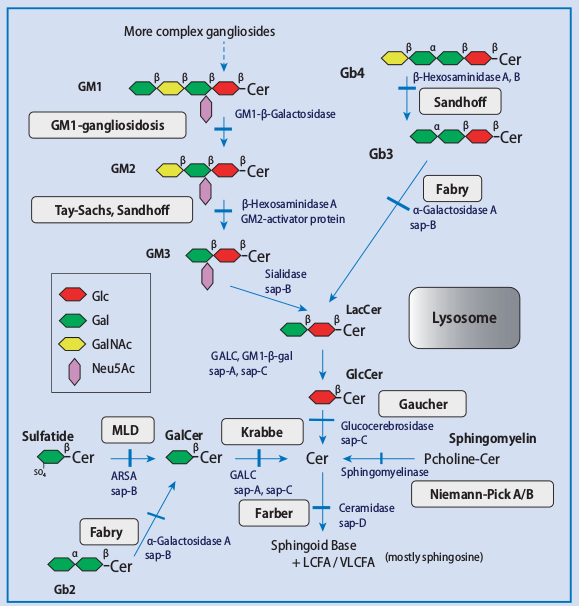
\includegraphics[width=0.8\textwidth]{./figures/sl_degradation.png}
\caption{\label{fig:orgeedca76}Sphingolipid Degradation}
\end{figure}

\subsection{Protein Trafficking to Lysosomes}
\label{sec:orgaf9b367}
\begin{itemize}
\item lysosomes are composed of soluble and transmembrane proteins that
are targeted to lysosomes in a signal-dependent manner
\item majority of soluble acid hydrolases are modified with mannose
6-phosphate (M6P) residues, allowing their recognition by M6P
receptors in the Golgi complex and ensuing transport to the
endosomal/lysosomal system
\item other soluble enzymes and non-enzymatic proteins are transported to
lysosomes in an M6P-independent manner mediated by alternative
receptors such as the lysosomal integral membrane protein LIMP-2 or
sortilin
\item sorting of cargo receptors and lysosomal transmembrane proteins
requires sorting signals present in their cytosolic domains
\item phosphorylation and lipid modifications regulate signal recognition
and trafficking of lysosomal membrane proteins
\end{itemize}

\begin{figure}[htbp]
\centering
\includegraphics[width=0.9\textwidth]{./figures/protein_trafficking.jpg}
\caption{\label{fig:org44a4a8e}Protein Trafficking to Lysosome}
\end{figure}

\begin{figure}[htbp]
\centering
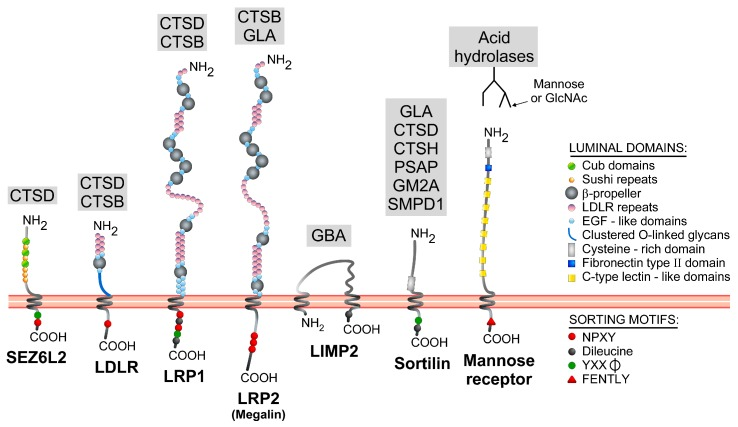
\includegraphics[width=0.8\textwidth]{./figures/lysosome_trafficking.jpeg}
\caption{\label{fig:orgc6ac8b9}Lysosomal Protein Trafficking Receptors}
\end{figure}

\subsubsection{M6P receptors}
\label{sec:org65e4509}
\begin{itemize}
\item MPRs are transmembrane glycoproteins that target enzymes to lysosomes in vertebrates
\item MPRs bind newly synthesized lysosomal hydrolases in the TGN and deliver them to pre-lysosomal compartments
\item there are two different MPRs
\begin{itemize}
\item the cation-independent mannose 6-phosphate receptor (CI-MPR)
\item CD-MPR requires divalent cations to efficiently recognize lysosomal hydrolases
\end{itemize}
\item bind terminal M6-P with similar affinity
\end{itemize}

\subsubsection{Sortilin}
\label{sec:org20c91e7}
\begin{itemize}
\item sortilin is a type I transmembrane protein found in lysosomes
\begin{itemize}
\item can transport several lysosomal proteins from the TGN or PM to the endosomes
\end{itemize}
\item tissues from sortilin knock-out mice exhibit normal morphology
\item sortilin may transport selected acid hydrolases in:
\begin{itemize}
\item a subset of cell types
\item under stress conditions (e.g. M6P pathway is deficient)
\end{itemize}
\end{itemize}

\subsubsection{LIMP-2}
\label{sec:orgd7b7988}
\begin{itemize}
\item LIMP-2 in a membrane protein in lysosomes that functions to regulate lysosomal/endosomal transport.
\item type III glycoprotein that is located primarily in limiting membranes of lysosomes and endosomes.
\item may participate in membrane transportation and the reorganization of endosomal/lysosomal compartment.
\end{itemize}

\subsubsection{Megalin}
\label{sec:orgb48cded}
\begin{itemize}
\item a cell surface receptor involved in reabsorption of proteins at the kidney proximal tubule
\item megalin mediated endocytosis of \(\alpha\)-galactosidase kidney proximal tubule
\item megalin also mediates the endocytosis of \(\alpha\)-galactosidase in renal podocytes
\end{itemize}

\subsection{Gaucher}
\label{sec:org9a9f027}
\subsubsection{Introduction}
\label{sec:org485db97}
\begin{itemize}
\item defect in \textbf{\(\beta\)-glucocerebrosidase (AKA: acid \(\beta\)-glucosidase)}
\begin{itemize}
\item extremely rare \textbf{SAP-C} deficiency
\end{itemize}
\item located in the lumen of lysosomes
\item LIMP-2 is responsible for MPR independent lysosomal targeting of
\(\beta\)-glucocerebrosidase
\item caused by accumulation of \textbf{glucocerebroside} the Gaucher lipid
\item most common LSD
\begin{itemize}
\item 1:40,000 to 1:50,000 live births
\end{itemize}
\item three types:
\begin{description}
\item[{Type 1}] no neurological symptoms
\item[{Type 2}] acute neuronopathic
\item[{Type 3}] sub-acute or chronic neuronopathic
\end{description}
\item Type 1 disease is common in Western Europe, the Americas and Israel
\item many other countries neuronopathic forms of Gaucher disease predominate
\end{itemize}

\begin{figure}[htbp]
\centering
\includegraphics[width=0.5\textwidth]{gaucher/figures/glucocerebroside.png}
\caption{\label{fig:org77c97fd}Glucocerebroside the Gaucher Lipid}
\end{figure}

\begin{figure}[htbp]
\centering
\includegraphics[width=0.5\textwidth]{gaucher/figures/glucocerebrosidase.png}
\caption{\label{fig:orgf5b9fba}\(\beta\)-Glucocerebrosidase: Gaucher}
\end{figure}

\subsubsection{Clinical Findings}
\label{sec:org7c913a1}
\begin{itemize}
\item see table \ref{tab:org81411c8}
\end{itemize}

\begin{table}[htbp]
\caption{\label{tab:org81411c8}Gaucher Clinical Variants}
\centering
\begin{tabular}{llll}
 & Type 1 & Type 2 & Type 3\\
\hline
Onset & Infant/Child/Adult & 3-6 months & Childhood\\
Neurodegeneration & Absent & \texttt{++++} & \texttt{++} \(\to\) \texttt{++++}\\
Survival & 6 - 80+ years & < 2 years & 2nd - 4th decade\\
Splenomegaly & \texttt{++++} & \texttt{++} & \texttt{++}\\
Hepatomegaly & \texttt{++} & \texttt{++} & \texttt{+}\\
Fractures, bone crises & \texttt{+} & - & \texttt{+}\\
Enrichment & Ashkenazi & None & Norrbottnian\\
 &  &  & Swedish\\
\end{tabular}
\end{table}

\begin{enumerate}
\item Gaucher Type 1
\label{sec:org77ab370}
\begin{itemize}
\item no neurological symptoms
\item clinical manifestations of Gaucher Type 1 are linked to macrophages
engorged with glucocerebroside

\item an undefined mechanism results in:
\begin{itemize}
\item enlargement and dysfunction of the liver and spleen
\item displacement of normal bone marrow by storage cells
\item osteoclastic-osteoblastic imbalances
\begin{itemize}
\item subsequent damage leading to bone infarctions and fractures
\end{itemize}
\item occasionally, involvement of other organs (e.g. lung) contributes
to the overall clinical picture
\item hypermetabolism and cachexia can be present
\item thrombocytopenia is the most common peripheral blood abnormality
\item a high incidence of Parkinsonism
\item spinal cord and nerve root compression
\end{itemize}
\end{itemize}

\item Gaucher Type 2
\label{sec:org012edd2}
\begin{itemize}
\item acute neuronopathic
\item Type 2 is the rarer of the two classic neuronopathic variants
\item early infantile onset of acute neuronopathic disease
\item progressing rapidly to death before age 2 years
\begin{itemize}
\item retroflexion of the neck
\item developmental delay, poor weight gain
\item protuberant abdomen due to hepatosplenomegaly
\item bulbar signs are prominent including:
\begin{itemize}
\item convergent squint, ocular paresis, trismus, dysphagia
\end{itemize}
\end{itemize}
\item perinatal-lethal subtype is the most severe form of Gaucher
disease
\begin{itemize}
\item \(\to\) death \emph{in utero} or hours to days after birth
\end{itemize}
\end{itemize}

\item Gaucher Type 3
\label{sec:org81cb429}
\begin{itemize}
\item sub-acute or chronic neuronopathic
\item Type 3 disease has a later onset, with slower progression of
neurologic manifestations and variable degrees of systemic
involvement
\item phenotype in Type 3 disease is considerably more
heterogeneous than that in Type 2
\item onset of symptoms occurs later, and neurologic involvement
progresses more slowly
\item includes abnormalities in:
\begin{itemize}
\item eye movements, seizures, intellectual deterioration
\end{itemize}
\item the same systemic manifestations occur as in Type 1 disease
\begin{itemize}
\item Type 3 patients may be incorrectly classified as Type 1 when
first seen
\end{itemize}
\end{itemize}
\end{enumerate}

\subsubsection{Genetics}
\label{sec:org8e73e7f}
\begin{itemize}
\item AR GBA or rarely PSAP (sap-C)
\item most of the >300 disease alleles in Gaucher disease are missense
mutations
\item genotype/phenotype correlations exist for:
\begin{itemize}
\item Type 1 disease (N370S)
\item Types 2 and 3 (L444P)
\end{itemize}
\item within these categories there is variable penetrance and
expressivity between individuals and ethnic groups
\end{itemize}
\subsubsection{Laboratory Investigations}
\label{sec:org9e7a95f}
\begin{figure}[htbp]
\centering
\includegraphics[width=0.6\textwidth]{gaucher/figures/Gaucher_Cells_with_Fibrillar_Appearing_Cytoplasm.jpg}
\caption{\label{fig:org1068c53}Gaucher Cells in a Bone Marrow Smear}
\end{figure}

\begin{enumerate}
\item Biochemistry
\label{sec:org9227b7e}
\begin{itemize}
\item \(\beta\)-glucocerebrosidase activity in:
\begin{itemize}
\item peripheral blood lymphocytes/leukocytes
\item dried blood spots
\item 4MU-\(\beta\)-D-glucopyranoside substrate
\end{itemize}
\item \(\uparrow\) chitotriosidase activity in serum or plasma 
\begin{itemize}
\item diagnosis and monitoring
\item CHIT1 genotype required due to common null CHIT1 allele
\item best monitoring biomarker
\end{itemize}
\item \(\uparrow\) acid phosphatase in serum and tissue 
\begin{itemize}
\item a lysosomal enzyme
\end{itemize}
\item \(\uparrow\) angiotensin converting enzyme in plasma
\begin{itemize}
\item not specific
\end{itemize}
\end{itemize}

\item Molecular
\label{sec:org963905c}
\begin{itemize}
\item GBA gene sequencing >300 disease alleles
\item C44P homozygotes have severe visceral disease, highly predisposed to
the development of CNS disease
\item N370S mutant enzyme appears to preclude the development of classical CNS disease of Gaucher disease
\item D409H mutation manifests a characteristic phenotype
\begin{itemize}
\item cardiac calcification, oculomotor apraxia, and corneal opacities
\end{itemize}
\end{itemize}
\end{enumerate}

\subsubsection{Treatment}
\label{sec:org75bf252}
\begin{enumerate}
\item Bone marrow transplantation
\label{sec:org30b0852}
\begin{itemize}
\item curative for Type 1
\begin{itemize}
\item suggests hematopoietic gene therapy
\end{itemize}
\item high risk of mortality
\end{itemize}
\item ERT
\label{sec:org71a5098}
\begin{itemize}
\item treats: hematological, visceral, and bony disease
\begin{itemize}
\item not cerebral disease
\end{itemize}
\item macrophages have a mannose receptor
\begin{itemize}
\item glucocerebrosidase glycoprotein modified to expose terminal mannose
\begin{description}
\item[{Ceredase (algucerase)}] human placenta, 1991
\item[{Cerezyme (imiglucerase)}] CHO cells, 1994
\item[{VPRIV (velaglucerase)}] human fibroblasts, 2010
\end{description}
\end{itemize}
\end{itemize}

\item Substrate reduction therapy
\label{sec:orgd27e050}
\begin{itemize}
\item miglustat an iminosugar a synthetic analogue of D-glucose
\begin{itemize}
\item inhibits ceramide glucoyltransferase required for synthesis of
glycosphingolipids
\item also used in Niemann-Pick C
\end{itemize}

\item isofagomine is a chaperone to stabilize missense mutation
\end{itemize}
\end{enumerate}

\subsection{Niemann-Pick  A \& B}
\label{sec:org2a6e08d}
\subsubsection{Introduction}
\label{sec:org7c65426}
\begin{itemize}
\item Niemann-Pick Type A and B are caused by deficiency of \textbf{acid sphingomyelinase (ASM)}
\begin{itemize}
\item acid sphingomyelinase is required to metabolize sphingomyelin
\item results in progressive \textbf{accumulation of sphingomyelin} in systemic organs
\begin{itemize}
\item brain accumulation in neuronal forms
\end{itemize}
\item NPA \& NPB represent opposite ends of a continuum
\begin{description}
\item[{NPA}] \textless{} 1\% of normal ASM
\item[{NPB}] \textasciitilde{} 10\% of normal ASM
\end{description}
\end{itemize}
\item lysosomal trafficking of acid sphingomyelinase is mediated by
sortilin and MPR
\begin{itemize}
\item MPR alone is sufficient to transport NPC2 to the endo/lysosomal compartment
\end{itemize}
\item incidence of Niemann-Pick A among Ashkenazi Jews \textasciitilde{} 1:40,000
\item incidence of both Niemann-Pick A and B in all other populations \textasciitilde{} 1:250,000
\end{itemize}

\begin{figure}[htbp]
\centering
\includegraphics[width=0.6\textwidth]{niemann_pick/figures/sphingomyelin.png}
\caption{\label{fig:org83f5e9f}Sphingomyelin}
\end{figure}

\begin{figure}[htbp]
\centering
\includegraphics[width=0.5\textwidth]{niemann_pick/figures/sphingomyelinase.png}
\caption{\label{fig:org1a56c25}Acid Sphingomyelinase: NP A \& B}
\end{figure}

\subsubsection{Clinical Findings}
\label{sec:org1131bfa}
\begin{enumerate}
\item Niemann-Pick A symptoms
\label{sec:orgccc14ea}
\begin{itemize}
\item fatal 1.5-3 years
\item hepatosplenomegaly by age 3 months
\item failure to thrive
\item psychomotor regression at 1 year
\begin{itemize}
\item progressive loss of mental and physical abilities
\end{itemize}
\item interstitial lung disease resulting in lung infections and lung failure
\item \textbf{cherry-red spot identified with eye examination (100\%)}
\end{itemize}
\item Niemann-Pick B symptoms
\label{sec:org9b5443d}
\begin{itemize}
\item normal intelligence and life-span
\item symptoms outlined under NPA (but less severe)
\item thrombocytopenia
\item short stature
\item \textbf{cherry-red spot identified with eye examination (50\%)}
\end{itemize}
\end{enumerate}

\subsubsection{Genetics}
\label{sec:orgebdd666}
\begin{itemize}
\item AR SMPD1
\item good phenotype-genotype correlation
\end{itemize}
\subsubsection{Diagnostic Tests}
\label{sec:orgd40410d}
\begin{itemize}
\item \(\Downarrow\) ASM activity in leukocytes or cultured cells
\begin{itemize}
\item use of native or radio-labelled substrate preferred to fluorescent substrate
\begin{itemize}
\item 6-hexadecanoylamino-4-methylumbelliferyl-phosphorylcholine
\begin{itemize}
\item does not detect Q292K mutation
\end{itemize}
\end{itemize}
\end{itemize}
\item \(\uparrow\) chitotriosidase activity
\item \(\uparrow\) lyso-sphingomyelin in dried blood spots
\item \(\uparrow\) plasma oxysterols
\begin{itemize}
\item oxysterols cholestane-3\(\beta\), 5\(\alpha\), 6\(\beta\)-triol
\item 7-ketocholesterol
\end{itemize}
\item atherogenic lipid profile 
\begin{itemize}
\item \(\uparrow\) cholesterol
\item \(\uparrow\) LDL cholesterol
\end{itemize}
\item foam cells in bone marrow (Figure \ref{fig:org21aa9fd})
\end{itemize}

\begin{figure}[htbp]
\centering
\includegraphics[width=0.25\textwidth]{niemann_pick/figures/foam_cells.png}
\caption{\label{fig:org21aa9fd}Foam Cells in Bone Marrow in NP A, B and C}
\end{figure}

\subsubsection{Treatment}
\label{sec:org6cd786b}
\begin{itemize}
\item no approved treatments
\item olipudase alfa - recombinant human acid sphingomyelinase (ASM) ERT
\begin{itemize}
\item treatment of nonneurologic manifestations
\item ongoing study to assessed safety and efficacy
\end{itemize}
\end{itemize}

\subsection{GM1 Gangliosidoses}
\label{sec:org37cf63f}
\subsubsection{Introduction}
\label{sec:orgb22da10}
\begin{itemize}
\item defect in \textbf{\(\beta\)-galactosidase (AKA: \(\beta\)-gangliosidase)}
\begin{itemize}
\item removes galactose from GM1, keratin sulfate and some oligosaccharides (Figure \ref{fig:orgb5df238})
\end{itemize}
\item \textbf{GM1 ganglioside accumulates in the brain and visera}
\item infantile, juvenile and adult forms
\begin{itemize}
\item correspond with amount of residual enzyme function
\item devastating degenerative disease
\end{itemize}
\item GM1 gangliosidosis of all types is estimated to occur in 1:100,000 - 300,000
\item GLB1-related disorders comprise two phenotypically distinct lysosomal storage disorders:
\begin{enumerate}
\item GM1 gangliosidosis
\item mucopolysaccharidosis type IVB (Morquio B)
\end{enumerate}
\item MPS IVB - Morquio B
\begin{itemize}
\item clinically indistinguishable from MPS IVA 
\begin{itemize}
\item skeletal changes, including short stature and skeletal dysplasia
\item normal intelligence
\end{itemize}
\item prevalence of MPS IVB has been reported as 1:250,000 - 1,000,000
\end{itemize}
\end{itemize}

\begin{figure}[htbp]
\centering
\includegraphics[width=0.4\textwidth]{GM1_2/figures/bgalatosidase.png}
\caption{\label{fig:orgb5df238}\(\beta\)-Galactosidase: GM1 Gangliosidosis}
\end{figure}


\begin{enumerate}
\item Lysosomal multi-enzyme complex
\label{sec:org21d8da6}
\begin{itemize}
\item \(\beta\)-galactosidase forms a heterotrimeric complex with cathepsin A
and neuraminidase
\item \(\downarrow\) cathepsin A \(\to\) 2\degree  deficiency of neuraminidase
\begin{itemize}
\item ML-1 (sialidosis) see Mucolipidosis
\end{itemize}
\end{itemize}
\end{enumerate}

\subsubsection{Clinical Findings}
\label{sec:org370ee66}
\begin{itemize}
\item see table \ref{tab:org8311946}
\item a cause of non-immune fetal hydrops
\end{itemize}
\begin{table}[htbp]
\caption[GM1 Signs and Symptoms]{\label{tab:org8311946}GM1 Signs and Symptoms}
\centering
\begin{tabular}{lllll}
Finding & Infantile & Juvenile & Adult & MPS IVB\\
\hline
onset of symptoms & <1 year & 1-10 years & 10+ years & 3-5 years\\
eye findings & CRS & CC\footnotemark & \pmCC & CC\\
motor abnormalities & + & + & extra pyramidal & \footnotemark\\
hepatosplenomegaly & + & \textpm{} & - & -\\
cardiac involvement & \textpm{} & \textpm{} & \textpm{} & +\\
coarse facial features & \textpm{} & - & - & \textsuperscript{\ref{org3ef6a97}}\\
skeletal findings & + & \textpm{} & - & +\\
urine & \footnotemark & \textsuperscript{\ref{org660e602}} & \textsuperscript{\ref{org660e602}} & keratan sulfate \footnotemark\\
 &  &  &  & \\
\end{tabular}
\end{table}\footnotetext[1]{\label{org9532b1c}corneal clouding}\footnotetext[2]{\label{org3ef6a97}secondary to bony changes}\footnotetext[3]{\label{org660e602}oligosacaride with terminal galactose}\footnotetext[4]{\label{org0b78a8e}FN have been observed}

\subsubsection{Genetics}
\label{sec:org08224a9}
\begin{itemize}
\item AR GLB1
\item \textasciitilde{} 150 mutations in GLB1 have been described
\item neither the type or location correlate with phenotype
\end{itemize}
\subsubsection{Laboratory Investigations}
\label{sec:orgb9b7c29}
\begin{itemize}
\item \(\beta\)-galactosidase activity: leukocytes and DBS
\begin{itemize}
\item 4-MU-\(\beta\)-d-galactopyranoside
\end{itemize}
\item \(\uparrow\) urine oligosacarides with terminal galactose
\item \(\uparrow\) urine keratin sulfate
\end{itemize}

\subsubsection{Treatment}
\label{sec:org6b4bb8e}
\begin{itemize}
\item no curative treatment to date
\end{itemize}
\subsection{GM2 Gangliosidoses}
\label{sec:org162b620}
\subsubsection{Introduction}
\label{sec:org2e82473}
\begin{itemize}
\item \textbf{\(\beta\)-hexosaminidase A} deficiency 
\begin{itemize}
\item impaired lysosomal catabolism of GM2 ganglioside
\end{itemize}
\item progressive cerebral degeneration
\item functional lysosomal \(\beta\)-hexosaminidase enzymes are dimeric
\begin{itemize}
\item three isozymes are produced through the combination of \(\alpha\)
and \(\beta\) subunits (Table \ref{tab:org6c2c7b9})
\end{itemize}
\end{itemize}

\begin{table}[htbp]
\caption{\label{tab:org6c2c7b9}Hexoaminidase Isozymes}
\centering
\begin{tabular}{lll}
Isozyme & Dimer composition & Function\\
\hline
A & \(\alpha\)/\(\beta\) & hydrolyzes GM2 ganglioside\\
B & \(\beta\)/\(\beta\) & non-GM2 gangliosides w terminal hexosamine\\
S & \(\alpha\)/\(\alpha\) & no known physiological function\\
\end{tabular}
\end{table}

\begin{itemize}
\item \(\beta\)-galactosidase, hexoaminidase A and B require the M6P-receptor
\begin{itemize}
\item secreted in ML II (I cell disease)
\end{itemize}
\item GM2 activator protein - sortilin

\item three genetic and biochemical subtypes
\begin{description}
\item[{Tay-Sachs disease}] \(\alpha\)-subunit \(\to\) Hex A deficiency
\item[{Sandhoff disease}] \(\beta\)-subunit \(\to\) Hex A\&B deficiencies
\item[{GM2 activator deficiency}] activator \(\to\) AB variant
\end{description}
\item GM2 storage in neurons in Tay-Sachs and Sandhoff
\begin{itemize}
\item Sandhoff \(\uparrow\) asialo-GM2 in brain, globoside and oligosacarides in viseral organs
\end{itemize}
\end{itemize}


\begin{table}[htbp]
\caption{\label{tab:org9d3a031}GM2 ganglioside storage diseases}
\centering
\begin{tabular}{llrll}
Disorder & Onset & Death (y) & Enzyme & Gene\\
\hline
Tay-Sachs & 3-6 months & 2-4 & Hex A & HEXA\\
Juvenile GM2 & 2-6 years & 5-15 & Hex A & HEXA\\
Adult GM2 & 2 yrs-adult & variable & Hex A & HEXA\\
\hline
Sandhoff & 3-6 months & 2-4 & Hex A\&B & HEXB\\
AB variant & 3-6 months &  & Activator & GM2A\\
\end{tabular}
\end{table}

\begin{figure}[htbp]
\centering
\includegraphics[width=0.5\textwidth]{GM1_2/figures/hexosaminidasea.png}
\caption{\label{fig:org5c6dab8}Hexosaminidase A: Tay-Sachs}
\end{figure}


\begin{figure}[htbp]
\centering
\includegraphics[width=0.5\textwidth]{GM1_2/figures/hexosaminidaseab.png}
\caption{\label{fig:org63cb60b}Hexosaminidase A \& B:Sandhoff disease (GL-3 \& 4 equivalent to Gb3 \& 4)}
\end{figure}


\subsubsection{Clinical Findings}
\label{sec:org6a916fc}
\begin{itemize}
\item see table \ref{tab:orga89ee1d}
\end{itemize}
\begin{table}[htbp]
\caption{\label{tab:orga89ee1d}GM2 Signs and Symptoms}
\centering
\begin{tabular}{llll}
Finding & Infantile & Juvenile & Adult\\
\hline
onset of symptoms & <1 year & 2-10 years & 10+ years\\
eye findings & CRS, blindness & \textpm{} CRS & \\
movement & weakness & ataxia, dysarthria & dystonia, ataxia\\
neurological & startle response & seizures & psychosis\\
 & seizures &  & \\
\end{tabular}
\end{table}

\subsubsection{Genetics}
\label{sec:orgbf4d1ee}
\begin{itemize}
\item AR HEXA, HEXB and GM2A
\item > 130 mutations in HEXA
\begin{itemize}
\item \textasciitilde{} 3 alleles comprise \textasciitilde{}95\% of Askenazi Jewish disease alleles
\item good correlation with phenotype
\end{itemize}
\item > 40 mutations in HEXB
\item 6 in GM2A
\end{itemize}
\subsubsection{Laboratory Investigations}
\label{sec:org8b84fd3}
\begin{itemize}
\item \emph{in vitro} hexoaminidase activity: leukocytes, fibroblasts
\begin{itemize}
\item 4-MU-6-sulfo-\(\beta\)-glucosaminide
\item specific for the \(\alpha\) subunit
\end{itemize}
\item falsely normal results in Tay-Sachs female carriers
\item the direct assay of hexosaminidase A using the sulfated synthetic
substrate (4-MU-6-sulfo-\(\beta\)-glucosaminide) specific for the \(\alpha\)-subunit
is the method of choice
\item total hexosaminidases (A+B) using a synthetic fluorogenic substrate
allows the diagnosis of Sandhoff disease
\item differential assay of HexA using heat or acid inactivation does not
identify patients with the B1 variant (see Methods)
\item high residual activity is found in Sandhoff disease
\begin{itemize}
\item excess of hexosaminidase S (\(\alpha \alpha\)-dimer)
\end{itemize}
\item GM2 activator deficiency
\begin{itemize}
\item normal \emph{in vitro} hexosaminidase A activity
\item definitive diagnosis requires GM2A sequencing
\end{itemize}
\item urine oligosacarides
\item \(\uparrow\) CSF GM2 ganglioside
\item electron microscopic examination of a skin or conjunctiva biopsy
\begin{itemize}
\item concentric lamellated bodies in nerve endings
\end{itemize}
\end{itemize}
\subsubsection{Treatment}
\label{sec:orgd71161b}
\begin{itemize}
\item treat seizures
\item no curative treatment to date
\end{itemize}
\subsection{Krabbe}
\label{sec:org7e63e31}
\subsubsection{Introduction}
\label{sec:orge6f97f1}
\begin{itemize}
\item rapidly progressive CNS degenerative disease
\item Krabbe is both a \textbf{leukodystrophy} affecting white matter of the central
and peripheral nervous systems, and an LSD
\begin{itemize}
\item hypomyelinating leukodystrophy (degeneration of white matter)
\end{itemize}
\item incidence of 1:100,000 births
\item deficiency in \textbf{galactocerebrosidase (AKA:galactosylceramidase)} 
\begin{itemize}
\item catabolism of galactocerebroside, a major lipid in myelin, kidney, and epithelial cells of the small intestine and colon.
\item results in accumulation of galactocerebroside in pathognomonic globoid cells
\begin{itemize}
\item multinucleated microglia/macrophages seen in the white matter
\end{itemize}
\end{itemize}
\item accumulation of psychosine (galactosylspingosine) in oligodendrocytes and Schwann cells
\end{itemize}

\begin{figure}[htbp]
\centering
\includegraphics[width=0.9\textwidth]{krabbe/figures/beta-galactosidase.png}
\caption{\label{fig:org0febeb8}Galactocerebrosidase: Krabbe}
\end{figure}

\begin{itemize}
\item galactocerebrosidase is a lysosomal enzyme
\item hydrolyzes the galactose ester bonds of galactocerebroside, galactosylsphingosine, lactosylceramide, and monogalactosyldiglyceride
\item requires saposin A cofactor
\item lysosomal trafficking of galactocerebrosidase by the M6P receptor
\begin{itemize}
\item enzyme is secreted in ML II (I cell disease)
\end{itemize}
\end{itemize}

\begin{enumerate}
\item Saposin A Cofactor Deficiency
\label{sec:org7c6d8c5}
\begin{itemize}
\item atypical Krabbe disease due to \textbf{saposin A (Sap-A)} deficiency is
caused by mutation in the prosaposin gene (PSAP)
\item sphingolipid activator proteins (saposins A, B, C and D) are small
homologous glycoproteins derived from a common precursor protein
(prosaposin) encoded by a single gene
\item they are required for \emph{in vivo} degradation of sphingolipids with
short carbohydrate chains
\end{itemize}
\end{enumerate}

\subsubsection{Clinical Findings}
\label{sec:orgf2f6517}
\begin{itemize}
\item Krabbe disease is a spectrum from infantile to late-onset

\item \textbf{infantile-onset} (age <12 months)

\begin{itemize}
\item normal development in the first few months followed by rapid
severe neurologic deterioration
\item excessive crying to extreme irritability
\item feeding difficulties, gastroesophageal reflux disease
\item spasticity of lower extremities and fist clenching, with axial hypotonia
\item loss of acquired milestones: smiling, cooing, and head control
\item staring episodes
\item peripheral neuropathy
\item the average age of death is 2 years (8 months to 9 years)
\end{itemize}

\item \textbf{later-onset} (age >12 months)
\begin{itemize}
\item manifests after 12 months and as late as the seventh decade
\item slow development of motor milestones or loss of milestones
\begin{itemize}
\item sitting without support, walking, slurred speech
\end{itemize}
\item spasticity of extremities with truncal hypotonia
\item vision loss, esotropia
\item seizures
\item peripheral neuropathy
\end{itemize}

\item 85-90\% of symptomatic individuals with Krabbe disease diagnosed by
enzyme activity alone have infantile-onset disease
\begin{itemize}
\item 10-15\% have later-onset disease
\end{itemize}
\item NBS suggests that the proportion of individuals with later-onset
Krabbe disease is higher than previously thought
\end{itemize}

\subsubsection{Genetics}
\label{sec:org7efe476}
\begin{itemize}
\item AR GALC or rarely PSAP (sap-A)
\item recurrent 30 kb deletion extends from intron 10 to intron 17
\begin{itemize}
\item infantile onset disease in homozygotes
\end{itemize}
\end{itemize}

\subsubsection{Diagnostic Tests}
\label{sec:orge36d631}
\begin{itemize}
\item diagnosis suspected in a symptomatic proband based on clinical
findings and other supportive laboratory, neuroimaging, and
electrophysiologic findings, is established by:
\begin{itemize}
\item detection of deficient GALC enzyme activity in leukocytes
\item abnormal results require follow-up molecular genetic testing of GALC
\item elevated psychosine levels can also help establish the diagnosis
\end{itemize}

\item in an asymptomatic newborn with low GALC enzyme activity on dried
blood spot specimens on NBS urgent time-critical measurement of:
\begin{itemize}
\item blood psychosine levels
\item GALC molecular genetic testing
\item necessary to identify, before age 14 days, newborns with evidence
of infantile-onset Krabbe disease who are candidates for early
HSCT
\end{itemize}
\end{itemize}

\begin{figure}[htbp]
\centering
\includegraphics[width=0.8\textwidth]{krabbe/figures/NBS_follow_up.png}
\caption{\label{fig:org15a7f13}NBS Follow-up at Mayo}
\end{figure}

\begin{itemize}
\item \(\uparrow\) CSF protein
\item leukocytes galactocerebrosidase activity 
\begin{itemize}
\item 6-hexadecanoylamino-4-MU-\(\beta\)-d-galactopyranoside
\end{itemize}

\item \(\uparrow\) DBS psychosine
\begin{itemize}
\item an amphipathic lipid that partitions largely into cellular
membranes
\item second-tier assay for infants with reduced galactocerebrosidase activity
\item diagnose and monitor patients with Krabbe disease and Saposin A
cofactor deficiency
\end{itemize}
\end{itemize}

\begin{enumerate}
\item Treatment
\label{sec:orgf5231f4}
\begin{enumerate}
\item Treatment of manifestations
\label{sec:org0fcfff6}
\begin{itemize}
\item treatment of a child who is symptomatic before age six months is
supportive and focused on increasing the quality of life and
avoiding complications
\item older individuals treatment with HSCT is individualized based on
disease burden and manifestations
\end{itemize}

\item Prevention of primary manifestations
\label{sec:orgfb43e57}
\begin{itemize}
\item asymptomatic newborns identified by either prenatal/neonatal
evaluation because of a positive family history of Krabbe disease
or an abnormal NBS result undergo additional testing to identify
those with infantile-onset Krabbe disease
\begin{itemize}
\item those with laboratory findings consistent with infantile-onset
Krabbe disease are candidates for HSCT before age 30 days
\end{itemize}
\end{itemize}

\item Surveillance
\label{sec:orgee03165}
\begin{itemize}
\item monitor symptomatic individuals with Krabbe disease for
development of:
\begin{itemize}
\item hydrocephalus, swallowing difficulties and chronic
microaspiration, scoliosis, hip subluxation, and osteopenia,
decreased vision, and corneal ulcerations
\end{itemize}
\end{itemize}
\end{enumerate}
\end{enumerate}
\subsection{Metachromatic Leukodystropy}
\label{sec:org40170c9}
\subsubsection{Introduction}
\label{sec:org8793823}
\begin{itemize}
\item \textbf{arylsulfatase A} deficiency
\begin{itemize}
\item block in lysosomal degradation of sulfatide (AKA sulfated
galactocerebroside) and other sulfated glycolipids
\item sulfatide is presented to the enzyme arylsulfatase A (ASA) as a
1:1 complex with sap-B
\item deficiency of either ASA or sap-B can cause MLD
\item MPR required for lysosomal trafficking
\end{itemize}
\item metachromatic leukodystrophy (MLD) incidence between 1:40,000 and 1:170,000
\begin{itemize}
\item specific ethnic groups with higher frequency
\end{itemize}

\item sulfatide is component of the myelin sheath
\begin{itemize}
\item sulfatide:galactocerebroside ratio affects stability and
physiological properties of this membrane
\item \(\uparrow\) sulfatides in CNS and PNS \(\to\) demyelination
\item \(\uparrow\) sulfatide in the kidney \(\to\) sulfatide in urine
\end{itemize}
\item demyelinating leukodystrophy (degeneration of white matter)
\end{itemize}

\begin{figure}[htbp]
\centering
\includegraphics[width=0.7\textwidth]{mld/figures/asa.png}
\caption{\label{fig:org060c9c9}Arylsulfatase A: Metachromatic Leukodystrophy}
\end{figure}

\subsubsection{Clinical}
\label{sec:org95fb6d3}
\begin{itemize}
\item three forms: late infantile-onset, juvenile and adult
\item variants include:
\begin{itemize}
\item saposin B deficiency
\item multiple sulphatase deficiency (see Section \ref{sec:orga22e633})
\end{itemize}
\end{itemize}
\begin{enumerate}
\item Late-infantile
\label{sec:org4d2b8c6}
\begin{itemize}
\item onset 1-2 years
\item typical presenting findings include weakness, hypotonia, clumsiness, frequent falls, toe walking, and dysarthria
\item language, cognitive, and gross and fine motor skills regress
\item later signs include spasticity, pain, seizures, and compromised vision and hearing
\item final stages, children have tonic spasms, decerebrate posturing, and
general unawareness of their surroundings
\end{itemize}

\item Juvenile
\label{sec:org916703b}
\begin{itemize}
\item onset 6-8 years
\item decline in school performance and emergence of behavioral problems, followed by gait disturbances
\item progression is similar to but slower than in the late-infantile form
\end{itemize}

\item Adult
\label{sec:orgcc3effb}
\begin{itemize}
\item onset occurs \textgreater{} 16 years, sometimes not until the fourth or fifth decade
\item problems in school or job performance, personality changes, emotional lability, or psychosis
\item neurologic symptoms (weakness and loss of coordination progressing
to spasticity and incontinence) or seizures initially
predominate
\item peripheral neuropathy is common
\item disease course is variable, periods of stability and decline two to three decades
\item final stage is similar to earlier-onset forms
\end{itemize}
\end{enumerate}

\subsubsection{Genetics}
\label{sec:orgd3759e1}
\begin{itemize}
\item AR ARSA or rarely PSAP (sap-B)
\item relatively good genotype-phenotype correlation
\item two very frequent ARSA polymorphisms 
\begin{itemize}
\item loss of an N-glycosylation site
\item loss of a polyadenylation signal
\end{itemize}
\item result in reduction of the amount of enzyme and constitute the
molecular basis of \textbf{ASA pseudodeficiency}
\end{itemize}

\subsubsection{Diagnosis}
\label{sec:orgbb45e0a}
\begin{itemize}
\item ASA activity in leukocytes or fibroblasts
\begin{itemize}
\item p-nitrocatechol-sulfate
\end{itemize}
\item pseudodeficiency is a major pitfall
\begin{itemize}
\item homozygotes for a PD allele (1-2\% of the European population)
\item compound heterozygotes for a disease-causing MLD and a PD allele
have about 5-15\% of normal ASA activity
\begin{itemize}
\item no detectable clinical abnormality or pathology
\end{itemize}
\item \(\therefore\) deficient ASA activity is not diagnostic
\end{itemize}
\item \textbf{sulfatides in the urinary sediment circumvents the PD problem}
\item MLD and MSD patients excrete sulfatides
\begin{itemize}
\item \(\Uparrow\) late infantile and juvenile patients
\item \(\uparrow\) adult-onset type
\item within or slightly above the normal range in PD
\end{itemize}
\item prenatal testing of MLD by DNA analysis is preferred
\item another cause of erroneous interpretation of an ASA deficiency is
\textbf{multiple sulfatase deficiency (MSD)} due to a deficiency in the
formylglycine-generating enzyme (FGE) encoded by SUMF1
\item \textbf{whenever a deficiency of one sulfatase is found, it is mandatory to}
\textbf{systematically measure the activity of another one to exclude MSD}
\begin{itemize}
\item arylsulfatase B or iduronate-2-sulfatase
\end{itemize}
\item MLD patients with sap-B deficiency
\begin{itemize}
\item \emph{in vitro} ASA assay will not show a deficiency
\item sulfatides and globotriaosylceramide (Gb3) in urine are essential
\begin{itemize}
\item both lipids are elevated \textbf{combined MLD and Fabry pattern}
\end{itemize}
\item diagnosis requires PSAP molecular genetics
\end{itemize}
\end{itemize}
\subsubsection{Treatment}
\label{sec:orga54adc2}
\begin{itemize}
\item HSCT has been used
\item lentiviral hematopoietic stem cell gene therapy tested
\item clinical trial of intrathecal administration of rhASA is ongoing
\end{itemize}
\subsection{Fabry}
\label{sec:orgbd7ddb1}
\subsubsection{Introduction}
\label{sec:orgdf9f1ac}
\begin{itemize}
\item AKA: angiokeratoma corporis diffusum universale
\item second most common LSD
\item defect in \textbf{\(\alpha\)-galactosidase A (AKA ceramide trihexosidase)}
\begin{itemize}
\item cleaves terminal galactose from globotriaosylceramide (Gb3)
(Figure \ref{fig:orgf5b9fba})
\item requires sap-B for activity
\begin{itemize}
\item sap-B deficiency is a form of metachromatic leukodystrophy
\end{itemize}
\item accumulation of Gb3 in blood vessels and other tissues
\begin{itemize}
\item Gb3 is the Fabry lipid (Figure \ref{fig:orgd6023fb})
\end{itemize}
\item 3 to 20\% activity in hemizygote males
\item wide range of symptoms including kidney, heart, and skin symptoms
\item \(\uparrow\) Gb3 in kidney and blood group B antigenic glycosphingolipid
\end{itemize}
\item \(\alpha\)-galactosidase A uses both sortilin and mannose receptor
\begin{itemize}
\item not affected in ML II (I-cell)
\end{itemize}
\end{itemize}

\begin{figure}[htbp]
\centering
\includegraphics[width=0.3\textwidth]{fabry/figures/globotriaosylceramide.png}
\caption[Globotriaosylceramide]{\label{fig:orgd6023fb}Globotriaosylceramide (Gb3): The Fabry lipid}
\end{figure}

\begin{figure}[htbp]
\centering
\includegraphics[width=0.4\textwidth]{fabry/figures/galactosidaseA.png}
\caption[\(\alpha\)-galactosidase A]{\label{fig:orge556e39}\(\alpha\)-Galactosidase A: Fabry}
\end{figure}


\subsubsection{Clinical Findings}
\label{sec:orgb1d1a08}
\begin{itemize}
\item see table \ref{tab:org07d9e92}
\item postprandial pain or diarrhea
\begin{itemize}
\item may be sole complaint
\end{itemize}
\item degradation of interphalangeal joints
\item cerebrovascular - stroke, seizures
\item ocular lesions
\item angiokeratomas (Figure \ref{fig:org6d6f6b9})
\begin{itemize}
\item prominent on hip, buttocks and scrotum
\end{itemize}
\end{itemize}

\begin{figure}[htbp]
\centering
\includegraphics[width=0.6\textwidth]{fabry/figures/angiokeratomas.png}
\caption[Angiokeratomas of the skin]{\label{fig:org6d6f6b9}Angiokeratomas of the Skin}
\end{figure}

\begin{table}[htbp]
\caption{\label{tab:org07d9e92}Fabry Signs and Symptoms}
\centering
\begin{tabular}{ll}
Age & Signs\\
\hline
childhood & pain in extremities, fever, Fabry crisis \footnotemark\\
adolescence & angiokeratomas\\
adulthood & CNS, myocardial and pulmonary\\
middle age & renal failure, lymphedema\\
\end{tabular}
\end{table}\footnotetext[5]{\label{org50df802}induced by heat, cold, fatigue or emotional stress}

\subsubsection{Genetics}
\label{sec:org606487e}
\begin{itemize}
\item \textbf{XL GLA}
\item penetrance in female heterozygotes
\begin{itemize}
\item may be considered X-linked dominant
\end{itemize}
\item AR PSAP(B) required for enzyme activity
\end{itemize}
\subsubsection{Laboratory Investigations}
\label{sec:orgc9f687f}
\begin{enumerate}
\item Biochemistry
\label{sec:org901135c}
\begin{itemize}
\item \(\downarrow\) \(\alpha\)-galactosidase A activity in leukocytes
\begin{itemize}
\item fluorometric 4MU-\(\alpha\)-D-galactopyranoside substrate
\item LC-MS/MS
\item unreliable in females
\end{itemize}
\item \(\uparrow\) urine Gb3 LC-MSMS 
\begin{itemize}
\item hemizygote males and heterozygote females
\end{itemize}
\item \(\uparrow\) plasma lyso-Gb3 (globotriaosylsphingosine) LC-MSMS
\begin{itemize}
\item sensitive biomarker
\item useful in diagnosis and monitoring
\end{itemize}
\end{itemize}

\item Pathology
\label{sec:org6c4a300}
\begin{itemize}
\item widespread deposition of Gb3
\item vacuoles seen in variety of cells
\begin{itemize}
\item \(\uparrow\) endothelium of blood vessels
\end{itemize}
\end{itemize}

\begin{figure}[htbp]
\centering
\includegraphics[width=0.4\textwidth]{fabry/figures/Fabrys-disease.jpg}
\caption[Fabry EM]{\label{fig:orga7c63c9}EM Showing Lamellar Structure of Lysosomal Inclusions in Fabry Disease Renal Biopsy}
\end{figure}
\end{enumerate}

\subsubsection{Treatment}
\label{sec:orgaad22d5}
\begin{itemize}
\item alleviate pain
\begin{itemize}
\item chronic low dose of phenytoin
\item carbamazapine, gabapentin
\end{itemize}
\item dialysis or renal transplantation
\item long term experience with ERT
\begin{itemize}
\item agalsidase (alpha or beta)
\item reduces left ventricular hypertrophy
\item less effect on renal function
\item does not prevent progression
\end{itemize}
\item oral chaperone therapy - migalastat
\begin{itemize}
\item only for amenable mutations
\end{itemize}
\end{itemize}
\subsection{Farber}
\label{sec:org5e9cd31}
\subsubsection{Introduction}
\label{sec:orgb230372}
\begin{itemize}
\item Farber lipogranulomatosis is very rare and clinically heterogeneous
\begin{itemize}
\item often presents during infancy causing death within the 1st year
\item later onset cases (up to an adult age) have been described
\item as well as foetal forms
\end{itemize}
\item deficiency of \textbf{acid ceramidase} activity
\begin{itemize}
\item leads to the storage of ceramides in various organs
\end{itemize}
\end{itemize}
\subsubsection{Genetics}
\label{sec:orgb684707}
\begin{itemize}
\item AR ASAH1
\end{itemize}
\subsubsection{Clinical}
\label{sec:org21fdaab}
\begin{itemize}
\item most frequent signs are painful joint swelling, deformation and
contractures, periarticular subcutaneous nodules and hoarseness due
to laryngeal involvement
\item neurodegeneration
\item some patients mimics juvenile idiopathic arthritis
\item hepatomegaly and cherry-red spot may be present
\end{itemize}

\subsubsection{Diagnosis}
\label{sec:org893ad75}
\begin{itemize}
\item ASAH1 genetics
\item EM of nodule or of a skin biopsy
\begin{itemize}
\item inclusions with typical curvilinear bodies in histiocytes
\item banana bodies in Schwann cells
\end{itemize}
\end{itemize}

\subsubsection{Treatment}
\label{sec:org75ff902}
\begin{itemize}
\item none
\item HSCT trial with poor outcome
\end{itemize}
\section{Niemann-Pick C}
\label{sec:orgf963244}
\subsection{Introduction}
\label{sec:orgadd6a15}
\begin{itemize}
\item a fatal, neuro-degenerative disease that affects \textasciitilde{} 1:150,000
\begin{itemize}
\item sometimes referred to as childhood Alzheimer’s
\item extremely heterogeneous
\item biochemically, genetically and clinically distinct from Niemann-Pick A and B
\end{itemize}
\item accumulation of unesterified cholesterol, sphingomyelin, glycolipids in systemic organs
\item GM2 and GM3 accumulate in brain
\begin{itemize}
\item no increase in cholesterol
\end{itemize}
\item NPC has two sub types NP-C1 (95\%) and NP-C2 (5\%)

\item LDL cholesterol enters cells via endocytosis at the LDL receptor
\item delivered to the late-stage endosomes and lysosomes
\item hydrolyzed and released as free cholesterol
\item unesterified cholesterol is transported to the plasma membrane and the ER for recycling

\item in NP-C the LDL-cholesterol is trapped in lysosomes
\end{itemize}

\begin{figure}[htbp]
\centering
\includegraphics[width=0.6\textwidth]{niemann_pick/figures/cholesterol1.jpg}
\caption{\label{fig:orgc67aa56}Cholesterol Transport}
\end{figure}

\subsubsection{NPC1 \& NPC2}
\label{sec:org0d3fbfd}

\begin{figure}[htbp]
\centering
\includegraphics[width=0.5\textwidth]{niemann_pick/figures/Niemann-Pick-C-Brown-and-Goldstein.png}
\caption{\label{fig:org4a2f102}NPC1 \& NPC2}
\end{figure}

\begin{itemize}
\item NPC1 is a lysosomal membrane protein involved in transport in the endosomal-lysosomal system
\item NPC2 acts in cooperation with the NPC1
\item disruption of transport results in accumulation of cholesterol and glycolipids in lysosomes
\end{itemize}

\subsection{Clinical Findings}
\label{sec:org22654ab}
\begin{itemize}
\item onset of the disease can happen at any age
\begin{itemize}
\item often school age children
\item also adults
\end{itemize}

\item symptoms may include:
\begin{itemize}
\item jaundice at birth or shortly afterwards
\item hepatosplenomegaly
\item vertical supranuclear gaze palzy
\item ataxia, dystonia, dysarthria, dysphagia
\item cognitive dysfunction/dementia
\item cataplexy, tremors, seizures
\end{itemize}
\end{itemize}

\subsubsection{Neurological Forms}
\label{sec:orga30b2b2}
\begin{enumerate}
\item Early Infantile
\label{sec:orgaa6b027}
\begin{itemize}
\item pre-existing hepatosplenomegaly
\item delay in motor milestones 9m-2yrs
\item survival <6 years
\end{itemize}

\item Late Infantile
\label{sec:org780a2c0}
\begin{itemize}
\item classic NPC 60-70\% of cases
\item language delay
\item ataxia 3-5 yrs
\item cognitive dysfunction 6-12 yrs
\end{itemize}

\item Adult
\label{sec:org94db9d2}
\begin{itemize}
\item diagnosis 15->60yrs
\item insidious presentation
\item ataxia, dystonia, dysarthria, movement disorders
\item variable cognitive dysfunction
\item vertical gaze palzy common
\end{itemize}
\end{enumerate}

\subsection{Genetics}
\label{sec:org4e6658e}
\begin{itemize}
\item AR NPC1 (95\%) and NPC2 (5\%)
\end{itemize}
\subsection{Diagnostic Tests}
\label{sec:orgae60193}
\begin{itemize}
\item foamy and sea-blue histiocytes may be found in bone marrow aspirates
(Figure \ref{fig:org21aa9fd})
\item plasma and DBS
\begin{itemize}
\item lysosphingomylin
\item lysosphingomylin-509
\end{itemize}
\item filipin staining in cultured fibroblasts
\begin{itemize}
\item culture fibroblasts in an LDL-enriched medium
\item pathognomonic free cholesterol accumulation in lysosomes
\item \(\uparrow\) fluorescence from filipin staining of cholesterol in lysosomes 
\begin{itemize}
\item unequivocal results in \textasciitilde{} 85\% of patients
\end{itemize}
\end{itemize}
\end{itemize}


\begin{figure}[htbp]
\centering
\includegraphics[width=0.5\textwidth]{niemann_pick/figures/filipin.png}
\caption{\label{fig:orgcbe765c}Filipin Staining (red:filipin stains cholesterol in lysosomes), green:CellMask)}
\end{figure}

\subsection{Treatment}
\label{sec:org60d875d}
\begin{itemize}
\item substrate reduction therapy
\begin{itemize}
\item miglustat approved for treatment of neurological manifestations
\begin{itemize}
\item an iminosugar a synthetic analogue of D-glucose
\end{itemize}
\item inhibits ceramide glucoyltransferase required for synthesis of
glycosphingolipids
\item also used in Gaucher
\end{itemize}
\end{itemize}

\section{Neuronal Ceroid Lipofuscinoses}
\label{sec:orgdf02bf7}
\subsection{Introduction}
\label{sec:orga8dac03}
\begin{itemize}
\item NCLs are a group of inherited progressive neurodegenerative diseases
\begin{itemize}
\item among the most frequent in childhood
\end{itemize}
\item NCL is widely used in Europe, "Batten disease" is common in the USA
\item wide clinical diversity is a result of  wide genetic heterogeneity
\begin{itemize}
\item 13 different genes identified
\item five of them encode soluble proteins
\item others encode transmembrane proteins whose function and possible
interactions still remain incompletely understood
\end{itemize}
\item NCLs are now considered as lysosomal storage diseases, due to the
lysosomal accumulation of lipopigments and localisation of several
NCL proteins to the lysosome
\end{itemize}

\subsection{Clinical Presentation}
\label{sec:org8743327}
\begin{itemize}
\item characterised by progressive psychomotor retardation, seizures,
visual loss and early death
\item four main clinical forms based on age of onset and order of
appearance of clinical signs
\begin{enumerate}
\item infantile - common in southern europe
\item late infantile - common in southern europe
\item juvenile - anglo-saxon
\item adult - rare
\end{enumerate}
\item now included classification based on genetic loci
\end{itemize}

\subsection{Metabolic Derangement}
\label{sec:org59ce629}
\begin{itemize}
\item accumulation of autofluorescent ceroid lipopigments mainly in
neural tissues
\begin{itemize}
\item saposins A and C in infantile forms
\item subunit c of mitochondrial ATP synthase in late infantile and
juvenile forms
\item not disease causing they are secondary markers
\end{itemize}
\item many CLN proteins
\begin{itemize}
\item many in lysosome but also mitochondria, ER and vesicular membranes
\end{itemize}
\item role in autophagy and apoptosis
\begin{description}
\item[{CLN1}] palmitoyl protein thioesterase - S-fatty acylated protein degradation
\item[{CLN2}] tripeptide peptidase - lysosomal serine protease
\item[{CLN10}] cathepsin D - endopepidatase
\end{description}
\end{itemize}

\subsection{Genetics}
\label{sec:org0c550da}
\begin{itemize}
\item AR
\item adult form is AD
\end{itemize}
\subsection{Diagnostic Tests}
\label{sec:org99361ce}
\begin{itemize}
\item electrophysiological studies
\item EM tissue biopsy with vacuolated lymphocytes
\item WBC or fibroblast enzyme studies
\begin{itemize}
\item CLN1 or 2
\item cathepsin D
\end{itemize}
\end{itemize}

\subsection{Treatment}
\label{sec:orgb1a91da}
\begin{itemize}
\item symptomatic treatment
\item control seizures
\end{itemize}
\section{Mucopolysaccharidoses}
\label{sec:orga22e633}
\subsection{Introduction}
\label{sec:org23567f7}
\begin{figure}[htbp]
\centering
\includegraphics[width=0.5\textwidth]{mps/figures/ch17f01.jpg}
\caption[Proteoglycans]{\label{fig:orgf2169c0}Proteoglycans}
\end{figure}

\begin{itemize}
\item proteoglycans are structural proteins of the ECM are embedded in gels formed from
proteoglycans
\item composed of glycosaminoglycans (GAGs) linked to a protein core
\item negatively charged GAGs bind Na\textsuperscript{+}
\begin{itemize}
\item draws water to create a gel
\end{itemize}
\item found in interstitial connective tissues such as: 
\begin{itemize}
\item synovial fluid
\item vitreous humour, cornea
\item arterial walls
\item bone, cartilage
\end{itemize}
\end{itemize}

\begin{figure}[htbp]
\centering
\includegraphics[width=0.5\textwidth]{mps/figures/ch3f1.jpg}
\caption[Proteoglycan Synthesis]{\label{fig:org87476e4}Proteoglycan Synthesis}
\end{figure}

\begin{figure}[htbp]
\centering
\includegraphics[width=0.8\textwidth]{mps/figures/snfg.png}
\caption[Glycan Nomenclature]{\label{fig:org2317580}Symbol Nomenclature for Glycans (SNFG)}
\end{figure}


\begin{figure}[htbp]
\centering
\includegraphics[width=0.6\textwidth]{mps/figures/ch17f02.jpg}
\caption[Glycosaminoglycans]{\label{fig:org863bbcc}Glycosaminoglycans}
\end{figure}

\begin{itemize}
\item GAGs are composed of repeating units of disaccharides (Figure \ref{fig:org863bbcc})
\begin{itemize}
\item hexosamine and a hexose or hexuronic acid
\end{itemize}
\end{itemize}
\begin{enumerate}
\item Hyaluronan
\label{sec:orge7114b4}
\begin{itemize}
\item composed of N-acetylglucosamine and glucuronate
\item not sulfated, not protein bound
\item forms in the plasma membrane instead of the Golgi
\item connective, epithelial, and neural tissues
\item cell proliferation and migration
\end{itemize}

\item Chondroitin Sulfate
\label{sec:orgf473b0d}
\begin{itemize}
\item composed of N-acetylgalactosamine and glucuronate
\item O-xylose-linked to core proteins
\item structural component of cartilage
\end{itemize}

\item Dermatan Sulfate
\label{sec:org80a4521}
\begin{itemize}
\item composed of N-acetylgalactosamine, glucuronate and iduronate
\item O-xylose-linked to core proteins
\item skin, blood vessels, heart valves, tendons, and lungs.
\item coagulation, cardiovascular disease, carcinogenesis, infection, wound repair, and fibrosis
\end{itemize}

\item Heparan Sulfate
\label{sec:orge3295f3}
\begin{itemize}
\item composed of glucosamine, iduronate, glucuronate and N-acetylglucosamine
\item O-xylose-linked to core proteins
\item developmental processes, angiogenesis, blood coagulation, tumour metastasis
\end{itemize}

\item Keratan Sulfate
\label{sec:orgf6ebf3a}
\begin{itemize}
\item composed of N-acetylglucosamine and galactose
\item KSI was isolated from corneal tissue and KSII from skeletal tissue
\item KSI is N-linked to specific asparagine amino acids via
N-acetylglucosamine
\item KSII is O-linked to specific serine or threonine amino acids via
N-acetyl galactosamine
\item cornea, cartilage, bone, CNS
\end{itemize}

\begin{figure}[htbp]
\centering
\includegraphics[width=0.6\textwidth]{mps/figures/ds_degradation_disorders.png}
\caption[DS Degradation]{\label{fig:orgbe5a2d7}Dermatan Sulfate Degradation}
\end{figure}

\begin{figure}[htbp]
\centering
\includegraphics[width=0.6\textwidth]{mps/figures/ks_degradation_disorders.png}
\caption[KS Degradation]{\label{fig:orgaaba034}Keratan Sulfate Degradation}
\end{figure}

\begin{figure}[htbp]
\centering
\includegraphics[width=0.5\textwidth]{mps/figures/hs_degradation_disorders.png}
\caption[HS Degradation]{\label{fig:org1815a45}Heparan Sulfate Degradation}
\end{figure}
\end{enumerate}

\subsection{Multiple Sulfatase Deficiency}
\label{sec:orgd663078}
\begin{itemize}
\item mutations in sulfatase modifying factor 1 (SUMF1) leading to a
deficiency in FGE (formylglycine-generating enzyme)
\item FGE is involved in the post-translational activation of all
sulfatases in the ER
\item deficiency leads to a deficiency of 17 sulfatases
\begin{itemize}
\item all lysosomal sulfatases including
\begin{itemize}
\item arylsulfatase A (MLD)
\item iduronate-2-sulfatase (Hunter)
\item heparin-N-sulfatase (Sanfilippo A)
\end{itemize}
\end{itemize}
\item MSD is very rare and clinical signs and symptoms are variable
\begin{itemize}
\item progressive psychomotor retardation invariably present
\end{itemize}
\item urine GAG concentrations can be normal
\begin{itemize}
\item \(\uparrow\) urine sulfatides
\item \(\downarrow\) measured \emph{in vitro} enzyme activity for multiple sulfatases
\end{itemize}
\end{itemize}

\subsection{Mucopolysaccharidoses}
\label{sec:org842233d}
\subsubsection{Clinical Presentation}
\label{sec:org618dfb5}
\begin{itemize}
\item all chronic, progressive and multisystem disorders
\item patients generally appear normal at birth
\begin{itemize}
\item accumulation of GAGs starts before birth and may lead to very
early symptoms such as:
\begin{itemize}
\item hydrops fetalis and intrauterine death (MPS VII)
\item skeletal deformities such as thoracolumbar kyphosis at birth (MPS IH)
\end{itemize}
\end{itemize}

\item important signs and symptoms in MPS include:
\begin{itemize}
\item dysostosis multiplex
\item bullet-shaped meta-carpals
\item oar-shaped ribs
\item facial dysmorphism
\item hepatosplenomegally
\item CNS disease
\item corneal clouding
\item cardiac valve thickening
\end{itemize}
\end{itemize}

\begin{table}[htbp]
\caption{\label{tab:org0eea3dc}MPS Signs and Symptoms}
\centering
\begin{tabular}{llllll}
MPS & variant & dysostosis & valvular & progressive & spinal cord\\
 &  & multiplex & heart disease & cognitive impairment & compression\\
\hline
MPS I & Hurler & \texttt{+++} & \texttt{+++} & \texttt{+++} & \texttt{+++}\\
 & Hurler-Scheie & \texttt{++} & \texttt{++} & \texttt{++} & \texttt{++}\\
 & Scheie & \texttt{++} & \texttt{++} & - & \texttt{++}\\
\hline
MPS II & neuronopathic & \texttt{++} & \texttt{++} & \texttt{+++} & \texttt{++}\\
 & attenuated & \texttt{++} & \texttt{++} & \textpm{} & \texttt{++}\\
\hline
MPS IIIA & Sanfilippo A & \texttt{+} & \textpm{} & \texttt{+++} & -\\
MPS IIIB & Sanfilippo B & \texttt{+} & \textpm{} & \texttt{+++} & -\\
MPS IIIC & Sanfilippo C & \texttt{+} & \textpm{} & \texttt{+++} & -\\
MPS IIID & Sanfilippo D & ? & ? & \texttt{+++} & -\\
\hline
MPS IVA & Morquio A & \texttt{+++} & \texttt{+} & - & \texttt{+++}\\
MPS IVB & Morquio B & \texttt{+++} & \texttt{+} & - & \texttt{+++}\\
\hline
MPS VI & Maroteaux-Lamy & \texttt{+++} & \texttt{+++} & - & \texttt{+++}\\
MPS VII & Sly & \texttt{+++} & \texttt{++} & \texttt{+++} & \texttt{+}\\
MPS IX &  & ? & ? & ? & ?\\
MSD & Austin & \texttt{++} & \texttt{+} & \texttt{+++} & ?\\
\end{tabular}
\end{table}

\begin{enumerate}
\item Dysmorphic syndrome
\label{sec:org0fee402}
\begin{itemize}
\item MPS I (Hurler)
\item MPS II (Hunter)
\item MPS VI (Maroteaux-Lamy)
\end{itemize}
\item Learning difficulties, behavioral disturbances and dementia
\label{sec:org29d3939}
\begin{itemize}
\item MPS III (Sanfilippo)
\end{itemize}
\item Severe skeletal dysplasia
\label{sec:orgcf0e0dc}
\begin{itemize}
\item MPS IV (Morquio)
\end{itemize}
\item Rare
\label{sec:org2311c2e}
\begin{itemize}
\item MPS VII (Sly)
\item MPS IX (Natowicz)
\end{itemize}
\end{enumerate}

\subsubsection{Metabolic Derangement}
\label{sec:orge95ea68}
\begin{itemize}
\item type of lysosomal storage disease
\item group of metabolic disorders caused by the absence or malfunctioning
of lysosomal enzymes needed to break down glycosaminoglycans (Table \ref{tab:org169cae8})
\item can be a result of decreased expression, stability, and activity of
one of the eleven enzymes required for glycosaminoglycans
degradation
\item GAGs collect in the cells, blood and connective tissues
\begin{itemize}
\item results in permanent, progressive cellular damage which affects:
\begin{itemize}
\item appearance
\item physical abilities
\item organ and system functioning
\item mental development in most cases
\end{itemize}
\end{itemize}
\end{itemize}

\begin{figure}[htbp]
\centering
\includegraphics[width=0.8\textwidth]{mps/figures/ch16f9.jpg}
\caption[Glycosaminoglycan Degradation]{\label{fig:org96d7c29}Glycosaminoglycan Degradation}
\end{figure}


\begin{table}[htbp]
\caption[Mucopolysaccharidoses]{\label{tab:org169cae8}MPS Enzymes and Substrates}
\centering
\begin{tabular}{lllll}
MPS & Name & Enzyme & GAG & Assay\\
\hline
MPS I & Hurler & \(\alpha\)-iduronidase & HS,DS & WBC\\
\hline
MPS II & Hunter & iduronate-2-sulfatase & HS,DS & plasma\\
\hline
MPS III & Sanfilippo A & heparan-N-sulfatase & HS & WBC\\
 & Sanfilippo B & N-acetyl glucosaminidase & HS & plasma\\
 & Sanfilippo C & \tiny{acetyl-CoA glucosamine N-acetyltransferase} & HS & WBC\\
 & Sanfilippo D & N-acetyl-glucosamine 6-sulfatase & HS & WBC\\
\hline
MPS IV & Morquio A & N-acetylgalactosamine 6-sulfatase & KS,CS & WBC\\
 & Morquio B\footnotemark & \(\beta\)-galactosidase & KS & WBC\\
\hline
MPS VI & Maroteaux-Lamy & N-acetylgalactosamine 4-sulfatase & DS & WBC\\
MPS VII & Sly & \(\beta\)-glucuronidase & DS,HS,CS & WBC\\
MPS IX &  & hyaluronidase & HA & fibro\\
MSD & Austin & formylglycine-generating enzyme & HS,DS & WBC\\
\end{tabular}
\end{table}\footnotetext[6]{\label{orgeb32972}\(\beta\)-galactosidase deficiency also causes GM1 gangliosidosis}

\subsubsection{Genetics}
\label{sec:orgd04f90c}
\begin{itemize}
\item AR
\item \textbf{MPS II Hunter is XLR}
\item see Lysosomal Storage Disorder Biochemistry table
\end{itemize}

\subsubsection{Diagnostic Tests}
\label{sec:orgc82186a}
\begin{itemize}
\item fractionation of urine GAGs (Table \ref{tab:org169cae8})
\begin{itemize}
\item dimethylmethylene blue dye binding assay (DMB) for total GAGs
quantitation
\item two-dimensional electrophoresis for fractionation excreted GAGs
\item false negatives reported
\item LC-MSMS method favoured
\end{itemize}
\item positive screen is followed by analysis of the relevant enzyme
activity in leukocytes or cultured skin fibroblasts
\begin{itemize}
\item enzymatic studies are the gold standard necessary to establish a
final diagnosis
\end{itemize}
\item Berry spot test lacks sufficient sensitivity and is obsolete for
screening for MPS
\begin{itemize}
\item urine applied to paper and stained with toluidine blue
\end{itemize}
\item \textbf{in a sulfatase deficiency, it is necessary to measure at least one}
\textbf{other sulfatase, in order to exclude multiple sulfatase deficiency}
\textbf{as the cause of the disease}
\end{itemize}

\subsubsection{Treatment}
\label{sec:orgfcfc1ff}
\begin{itemize}
\item symptomatic care
\item HSCT - MPS I, II, VI
\begin{itemize}
\item not effective in III and IVA
\end{itemize}
\item ERT - MPS I, II, IVA
\item IV ERT does not cross the blood–brain barrier
\begin{itemize}
\item no neurocognitive effect
\end{itemize}
\end{itemize}

\section{Oligosaccharidoses}
\label{sec:orgb519f2a}
\subsection{Introduction}
\label{sec:org67f9429}
\begin{itemize}
\item almost all the secreted and membrane associated proteins of the body
are glycosylated
\begin{itemize}
\item also numerous intracellular proteins such as lysosomal acid hydrolases
\end{itemize}
\item a variety of oligosaccharide chains are attached to the protein
backbone via:
\begin{itemize}
\item hydroxyl group of serine or threonine (O-linked)
\item amide group of asparagine (N-linked)
\end{itemize}
\item chains usually have a core composed of N-acetylglucosamine and mannose
\begin{itemize}
\item often contain galactose, fucose and N-acetylgalactosamine
\item frequently terminal sialic acids (N-acetylneuraminic acid)
\end{itemize}
\item oligosaccharide chains with a terminal mannose-6-phosphate are
involved in the targeting of lysosomal enzymes to lysosomes
\begin{itemize}
\item defects in synthesis of the M6P recognition marker \(\to\)
mislocalisation of lysosomal enzymes
\end{itemize}
\item deficiencies of the enzymes required for the degradation of the
oligosaccharide chains cause oligosaccharidoses
\end{itemize}



\begin{figure}[htbp]
\centering
\includegraphics[width=0.5\textwidth]{oligosaccharidoses/figures/oligosacch.png}
\caption{\label{fig:org5b40637}Glycoprotein Oligosaccharide Chain}
\end{figure}

\subsection{Oligosaccharidoses}
\label{sec:org4b0fcf5}
\subsubsection{Clinical Presentation}
\label{sec:orgb1b539f}
\begin{itemize}
\item oligosaccharidoses share many features in common with MPS disorders (Table \ref{tab:org4e3adaa})
\begin{itemize}
\item urine GAG screen is normal or only shows nonspecific
abnormalities
\end{itemize}
\end{itemize}

\begin{table}[htbp]
\caption{\label{tab:org4e3adaa}Oligosaccharidoses}
\centering
\begin{tabular}{lllllll}
Disease & Enzyme & dysostosis & progressive & angio- & hepato- & sample\\
 &  & multiplex & cognitive & keratoma & splenomegally & \\
\hline
\(\alpha\)-mannosidase & \(\alpha\)-mannosidase & \texttt{++} & \texttt{+} & - & \texttt{+} & WBC\\
\(\beta\)-mannosidase & \(\beta\)-mannosidase & \texttt{+} & \texttt{+++} & - & \texttt{+} & WBC\\
fucosidosis & fucosidase & \texttt{+} & \texttt{++} & \texttt{+++} & - & WBC\\
galactosialidosis & cathepsin A & \texttt{++} & \texttt{++} & - & \texttt{+} & Fib \& DNA\\
\end{tabular}
\end{table}

\begin{enumerate}
\item Mannosidosis
\label{sec:org6987eba}
\begin{itemize}
\item deficiency of \textbf{\(\alpha\)-mannosidase} \(\to\) variable disorder \(\alpha\)-mannosidosis
\item mild Hurler phenotype
\begin{itemize}
\item variable learning difficulties
\item hepatosplenomegaly
\item deafness
\item skeletal dysplasia
\end{itemize}
\item complicated by an immune deficiency which can dominate the clinical
progression of the disease

\item \(\beta\)-mannosidosis due to deficiency of \textbf{\(\beta\)-mannosidase}
\begin{itemize}
\item much less prevalent than \(\alpha\)-mannosidosis
\item very variable, but severe learning difficulties, challenging
behaviour, deafness and frequent infections are relatively common
\end{itemize}
\end{itemize}

\item Fucosidosis
\label{sec:org2f43216}
\begin{itemize}
\item lack the typical facial dysmorphism
\item deficiency of \textbf{\(\alpha\)-fucosidase} \(\to\) variable neurodegenerative disorder
\item often with seizures and mild dysostosis
\item often exhibit prominent and widespread angiokeratomas, progress with age
\end{itemize}

\item Galactosialidosis
\label{sec:org145b709}
\begin{itemize}
\item combined deficiency of the lysosomal enzymes \(\beta\)-galactosidase and
\(\alpha\)-neuraminidase
\item results from a defect in \textbf{protective protein/cathepsin A (PPCA)}
\begin{itemize}
\item an intralysosomal protein which protects these enzymes from
premature proteolytic processing
\end{itemize}
\item presentation varies from:
\begin{itemize}
\item hydrops fetalis
\item slowly progressive disorder associated with learning
difficulties, dysostosis multiplex and corneal opacity
\end{itemize}
\end{itemize}
\end{enumerate}

\subsubsection{Genetics}
\label{sec:org6333d2a}
\begin{itemize}
\item AR
\end{itemize}

\begin{table}[htbp]
\caption{\label{tab:org9cb1ee8}Oligosaccharidoses Genetics}
\centering
\begin{tabular}{lll}
Disease & Enzyme & Gene\\
\hline
\(\alpha\)-mannosidase & \(\alpha\)-mannosidase & MAN2B1\\
\(\beta\)-mannosidase & \(\beta\)-mannosidase & MANBA\\
fucosidosis & fucosidase & FUCA1\\
galactosialidosis & cathepsin A & PPCA\\
\end{tabular}
\end{table}

\subsubsection{Diagnostic Tests}
\label{sec:org17187a2}
\begin{itemize}
\item clinical suspicion
\item urine oligosaccharide excretion
\begin{itemize}
\item 1D TLC
\item treated with orcinol reagent and heated to 100\degreeC to visualize
\end{itemize}
\item usually normal urine GAGs
\item enzyme activity assays (Table \ref{tab:org4e3adaa})
\end{itemize}

\subsubsection{Treatment}
\label{sec:org1017348}
\begin{itemize}
\item supportive
\end{itemize}
\section{Mucolipidoses}
\label{sec:org4ca42c0}
\subsection{Introduction}
\label{sec:org656c818}
\begin{itemize}
\item mucolipidoses derived their name from the similarity in
presentation to both mucopolysaccharidoses and sphingolipidoses
\item four conditions have been labelled as mucolipidoses:
\begin{description}
\item[{ML I: sialidosis}] a glycoproteinosis
\item[{ML II: I-cell}] a glycoproteinosis
\item[{ML III: pseudo-Hurler polydystropy}] a glycoproteinosis
\item[{ML IV: ganglioside sialidase deficiency}] gangliosidosis
\end{description}
\end{itemize}


\begin{table}[htbp]
\caption{\label{tab:orgc89db12}Mucolipidoses}
\centering
\small
\begin{tabular}{lllllll}
Disease & Enzyme & dysostosis & progressive & angio- & hepato & sample\\
 &  & multiplex & cognitive & keratoma & -splenomegally & \\
\hline
ML I & \(\alpha\)-neuraminidase & \texttt{++} & \texttt{++} & - & \texttt{+} & fibro\\
ML II\&III & UDP-N-acetylglucosamine- & \texttt{+++} & \texttt{+} & - & - & plasma\\
 & 1-phosphotransferase &  &  &  &  & \\
ML IV & mucolipin-1 & - & \texttt{++} & - & - & DNA\\
\end{tabular}
\end{table}

\subsection{ML I (Sialidosis)}
\label{sec:org4f9073a}
\subsubsection{Clinical Presentation}
\label{sec:orgfc23b8f}
\begin{itemize}
\item Type I sialidosis is the milder form of this disorder
\begin{itemize}
\item development of ocular cherry-red spots and generalized
myoclonus in the second or third decade of life
\item \textgreater{} 50\% of patients have seizures, hyperreflexia, and ataxia
\end{itemize}

\item Type II sialidosis early onset of a progressive, severe, MPS-like
phenotype
\begin{itemize}
\item visceromegaly, dysostosis multiplex, and mental retardation
\end{itemize}
\end{itemize}

\subsubsection{Metabolic Derangement}
\label{sec:org8721d11}
\begin{itemize}
\item deficiency of \textbf{\(\alpha\)-neuraminidase} that normally cleaves terminal
\(\alpha\)2 \(\to\) 3 and \(\alpha\)2 \(\to\) 6 sialyl linkages of several
oligosaccharides and glycopeptides
\begin{itemize}
\item \(\therefore\) \(\uparrow\) oligosaccharides and glycopeptides in tissues
and fluids of affected patients
\end{itemize}
\end{itemize}

\subsubsection{Genetics}
\label{sec:org528ea2a}
\begin{itemize}
\item AR NEU1
\end{itemize}
\subsubsection{Diagnostic Tests}
\label{sec:org3c501d4}
\begin{itemize}
\item test urine samples for both oligosaccharides and glycopeptides
\item definitive diagnosis - measurement of sialidase activity in fresh
tissue samples
\begin{itemize}
\item fibroblasts, cultured amniotic fluid cells, or white blood cells
\end{itemize}
\end{itemize}

\subsubsection{Treatment}
\label{sec:org128794b}
\begin{itemize}
\item supportive
\end{itemize}

\subsection{ML II \& III}
\label{sec:org6a6cb68}
\begin{itemize}
\item ML II AKA: I-Cell Disease
\item ML III AKA: Pseudo-Hurler
\end{itemize}
\subsubsection{Clinical Presentation}
\label{sec:orgd603a08}
\begin{enumerate}
\item ML II
\label{sec:org74429d7}
\begin{itemize}
\item low IQ
\item short, max 75 cm by 2 y
\item early coarse features
\item gingival hypertrophy
\item limited joint movement
\item dysostosis multiplex
\item minimal to no hepatomegaly and splenomegaly
\end{itemize}

\item ML III
\label{sec:orgca7c9d5}
\begin{itemize}
\item pathology of ML-III is not well documented
\begin{itemize}
\item available data indicate the presence of similar but less severe
findings
\end{itemize}
\item ML-II and ML-III can be distinguished on clinical criteria and on
progression of the disease
\end{itemize}
\end{enumerate}

\subsubsection{Metabolic Derangement}
\label{sec:orgaf4be85}
\begin{itemize}
\item ML II and ML III result from a deficiency of the enzyme
N-acetylglucosamine-1-phosphotransferase
\begin{description}
\item[{ML II}] inactivity
\item[{ML III}] deficiency
\item \(\alpha \alpha \beta \beta \gamma \gamma\)-hexamer
\item phosphorylates target carbohydrate residues on N-linked
glycoproteins
\begin{itemize}
\item required for MPR mediated protein trafficking to lysosomes
\end{itemize}
\end{description}

\item characterized by deficient activity of a large number of lysosomal enzymes including:
\begin{description}
\item[{\(\beta\)-glucuronidase}] MPS VII
\item[{\(\beta\)-galactosidase}] GM1
\item[{\(\alpha\)-mannosidase}] mannosidosis
\item[{\(\alpha\)-fucosidase}] fucosidosis
\item[{arylsulfatase-A}] MLD
\item[{hexosaminidase A}] GM2
\end{description}
\item activities of the same lysosomal enzymes are high in the medium
surrounding cultured I-cell fibroblasts

\item I-cells are caused by oligosaccharides, lipids, and
glycosaminoglycan inclusions in lysosomes
\end{itemize}

\begin{table}[htbp]
\caption{\label{tab:orgb6717cd}Lysosomal Enzyme Receptors}
\centering
\begin{tabular}{lll}
Disease & Enzyme & Receptor\\
\hline
Gaucher & \(\beta\)-glucocerebrosidase & LIMP-2\\
Fabry & \(\alpha\)-galactosidase A & sortilin \& MPR\\
MLD & arylsulfatase A & MPR\\
GM1 & \(\beta\)-galactosidase & MPR\\
GM2 & hexosaminidase A and/or B & MPR\\
Krabbe & galactosylceramidase & MPR\\
NPA/B & acid sphingomyelinase & sortilin \& MPR\\
\end{tabular}
\end{table}



\begin{figure}[htbp]
\centering
\includegraphics[width=1\textwidth]{mucolipidosis/figures/lysosome_traffic.jpg}
\caption[Protein trafficking to lysosomes]{\label{fig:org5d8a9f0}Protein Trafficking to Lysosomes}
\end{figure}


\begin{figure}[htbp]
\centering
\includegraphics[width=1\textwidth]{mucolipidosis/figures/ml_defect.png}
\caption[N-acetylglucosamine (GlcNAc) phosphotransferase]{\label{fig:orga5681a5}N-acetylglucosamine (GlcNAc) Phosphotransferase}
\end{figure}

\begin{figure}[htbp]
\centering
\includegraphics[height=0.5\textwidth]{mucolipidosis/figures/icell.png}
\caption{\label{fig:org07ee84a}I-Cell in Fibroblast Culture}
\end{figure}

\subsubsection{Genetics}
\label{sec:org85e2808}
\begin{itemize}
\item AR GNPTAB
\end{itemize}

\subsubsection{Diagnostic Tests}
\label{sec:org1d9fd44}
\begin{itemize}
\item diagnosis is generally made by assay of lysosomal enzymes
\begin{itemize}
\item \(\Downarrow\) in cultured fibroblasts
\item \(\Uparrow\) in the plasma or serum
\begin{itemize}
\item 10- to 20-fold increase in enzyme activity
\end{itemize}
\end{itemize}
\item fibroblast or plasma glycosylasparaginase activity
\item fibroblast or leukocytes GlcNAc phosphotransferase activity
\end{itemize}

\subsubsection{Treatment}
\label{sec:org9841844}
\begin{itemize}
\item supportive
\end{itemize}
\subsection{ML IV}
\label{sec:org84184c2}
\subsubsection{Clinical Presentation}
\label{sec:orga0a669c}
\begin{itemize}
\item severe motor developmental delay
\item iron deficiency anemia
\item corneal clouding
\item progressive retinal degeneration
\item achlorhydria (\(\downarrow\) gastric secretions)
\item notably absent are dysplastic bone abnormalities and enlargement of
\end{itemize}
organs such as the liver and the spleen

\subsubsection{Metabolic Derangement}
\label{sec:org95cd1cb}
\begin{itemize}
\item inborn error of intracellular membrane trafficking due to mucolipin-1 deficiency
\begin{itemize}
\item unclear why  mucolipin-1 deficiency causes ML IV
\end{itemize}
\item associated with lysosomal inclusions in a variety of cell types
\end{itemize}
\subsubsection{Genetics}
\label{sec:orge816983}
\begin{itemize}
\item AR MCOLN1
\end{itemize}
\subsubsection{Diagnostic Tests}
\label{sec:org5bdc13c}
\begin{itemize}
\item \(\uparrow\) blood gastrin levels
\begin{itemize}
\item virtually diagnostic of ML IV with consistent clinical presentation
\end{itemize}
\item molecular
\end{itemize}

\subsubsection{Treatment}
\label{sec:orgbb776f4}
\begin{itemize}
\item supportive
\end{itemize}

\section{Peroxisomes}
\label{sec:orge0e3bad}
\subsection{Introduction}
\label{sec:org4ad3854}
\begin{itemize}
\item peroxisomes are required for \(\beta\)-oxidation of:
\begin{itemize}
\item very-long-chain fatty acids
\begin{itemize}
\item C22:6-CoA, C22:5-CoA, C26:1-CoA, C26:0-CoA
\item do not degrade fatty acids to completion
\end{itemize}
\item bile acid intermediates di- and trihydroxycholestanoic acid
\item a range of eicosanoids
\end{itemize}
\item \(\alpha\)-oxidation of phytanoyl-CoA \(\to\) pristanoly-CoA
\begin{itemize}
\item \(\beta\)-oxidation of pristanoly-CoA
\end{itemize}
\item single enzyme or transport protein defect result in abnormalities in some fatty acids
\end{itemize}

\begin{figure}[htbp]
\centering
\includegraphics[width=\textwidth]{peroxisomes/figures/non_mito_FA_met.png}
\caption{\label{fig:org1cdc324}Non-Mitochondrial FA Metabolism}
\end{figure}

\begin{itemize}
\item peroxisomal \(\beta\)-oxidation disorders
\begin{enumerate}
\item single peroxisomal enzyme or transport protein deficiencies
\begin{itemize}
\item X-Linked Adrenoleukodystrophy (X-ALD)
\item D-Bifunctional Protein (DBP) Deficiency
\item Acyl-CoA Oxidase (ACOX) Deficiency
\item Methyl Acyl-CoA Racemase (AMACR) Deficiency
\end{itemize}
\item generalized peroxisomal \(\beta\)-oxidation deficiencies
\begin{itemize}
\item Zellweger Spectrum disorders
\end{itemize}
\end{enumerate}
\item peroxisomal \(\alpha\)-oxidation disorders
\begin{itemize}
\item Refsum disease
\end{itemize}
\item Sjogren Larsson Syndrome
\item etherphospholipid biosynthesis
\begin{itemize}
\item Rhizomelic Chondrodysplasia Punctata (RCDP) 1-4
\end{itemize}
\item FA elongation disorders
\begin{itemize}
\item EVOL4, EVOL5
\item Trans-2,3-Enoyl-CoA Reductase (TER), 3-Hydroxyacyl-CoA Dehydratase 1 (HACD1)
\end{itemize}
\item eicosanoid metabolism
\begin{itemize}
\item Primary Hypertrophic Osteoarthropathy Type 1
\item LTC4-Synthase Deficiency
\end{itemize}
\end{itemize}


\begin{table}[htbp]
\caption{\label{tab:org784dab3}Biochemical Findings in Peroxisomal Disease}
\centering
\begin{tabular}{llllll}
Disease & VLCFA & plasmalogens & phytanic & pristanic & bile acids\\
\hline
ZS & \(\uparrow\) & \(\downarrow\) or N & \(\uparrow\) or N & \(\uparrow\) or N & \(\uparrow\) or N\\
RCDP & N & \(\downarrow\) & N or \(\uparrow\) & \(\downarrow\) or N & N\\
XALD & \(\uparrow\) & N & N & N & N\\
Refsum & N & N & \(\uparrow\) & \(\downarrow\) & N\\
\end{tabular}
\end{table}

\subsection{X-linked Adrenoleukodystrophy}
\label{sec:org09ccc6b}
\subsubsection{Clinical Presentation}
\label{sec:org866df18}
\begin{itemize}
\item three forms:
\begin{enumerate}
\item Childhood Cerebral Form
\begin{itemize}
\item more severe
\item neurological symptoms between 4-12 years
\item vegetative state and death
\item males may present with ADD or behavioural changes
\item followed by severe visual and hearing impairment, quadriplegia and
cerebellar ataxia
\end{itemize}
\item Adrenomyeloneuropathy (AMN) 
\begin{itemize}
\item 65\% of adult X-ALD male patients (20-50 years)
\item up to 88\% of heterozygous women (\textgreater{}40 years)
\item presentation is progressive spastic paraparesis and sensory ataxia
\end{itemize}
\item Addison Disease only
\begin{itemize}
\item primary adrenocortical insufficiency commonly by age 7.5 years
\item without evidence of neurologic abnormality
\begin{itemize}
\item some neurologic disability (most commonly AMN) usually
develops by middle age
\end{itemize}
\end{itemize}
\end{enumerate}
\end{itemize}

\subsubsection{Metabolic Derangement}
\label{sec:org8e8d2f6}
\begin{itemize}
\item deficiency in \textbf{ALDP a peroxisomal ABC transporter}
\begin{itemize}
\item required for import of VLCFAs (\textpm{} CoA) into peroxisomes
\begin{itemize}
\item \(\uparrow\) VLCFA-CoA in cytosol
\item incorporation into a variety of lipids including:
\begin{itemize}
\item cholesterol esters, phospholipids, and sphingolipids
\end{itemize}
\end{itemize}
\end{itemize}
\item VLCFAs accumulate in virtually all tissues, including erythrocytes,
white blood cells and plasma
\end{itemize}

\subsubsection{Genetics}
\label{sec:org567b776}
\begin{itemize}
\item \textbf{X-linked ABCD1}
\end{itemize}

\subsubsection{Diagnostic Tests}
\label{sec:org24f28ab}
\begin{itemize}
\item \(\downarrow\) cortisol and aldosterone
\item quantitative VLCFAs including: C22:0, C24:0, and C26:0 in plasma
\begin{itemize}
\item alkaline and acid hydrolysis releases the VLCFAs from all lipid
species
\item \(\uparrow\) concentration of C26:0
\item \(\uparrow\) C26:0/C22:0
\item \(\uparrow\) C24:0/C22:0
\begin{itemize}
\item C22:0 used as denominator \(\because\) not increased
\end{itemize}
\end{itemize}
\item normal plasma VLCFA does not exclude XALD in heterozygote females
\begin{itemize}
\item mutation analysis is the most reliable method for diagnosis in females
\end{itemize}
\item false-positive results have been reported in:
\begin{itemize}
\item patients on a ketogenic diet
\item recent ingestion of peanut butter
\end{itemize}
\item see table \ref{tab:org784dab3}
\end{itemize}
\subsubsection{Treatment}
\label{sec:orgf0d035d}
\begin{itemize}
\item a boy born with X-ALD has a 35\% risk of developing cerebral ALD
between the age of 4-12 years
\item 100\% risk of developing AMN between the age of 25-50 years
\item cerebral X-ALD can be treated in boys and adult males
\begin{itemize}
\item only at a very early stage of the disease
\item when patients start to develop cerebral demyelination on brain MRI
but have no or minimal neurologic symptoms
\end{itemize}
\item HSCT can arrest the cerebral demyelination when the procedure is
performed at a very early stage
\end{itemize}

\subsection{Zellweger Spectrum Disorders}
\label{sec:orgb9aab41}
\begin{itemize}
\item spectrum includes:
\begin{itemize}
\item Zellweger Syndrome
\item Neonatal Adrenoleukodystrophy (NALD)
\item Infantile Refsum Disease
\end{itemize}
\item once thought to be distinct disorders but are now considered to be
part of the same condition spectrum
\begin{itemize}
\item Zellweger Syndrome is the most severe form of the Zellweger Spectrum
\item NALD is intermediate in severity
\item IRD is the least severe form
\end{itemize}
\end{itemize}

\subsubsection{Clinical Presentation}
\label{sec:orge9f24cb}
\begin{enumerate}
\item Zellweger Syndrome
\label{sec:orgb716baf}
\begin{itemize}
\item presents in newborn period
\begin{itemize}
\item severe hypotonia, seizures
\item life-threatening dysfunction in organs and tissues
\begin{itemize}
\item liver, heart, and kidneys
\end{itemize}
\item may have skeletal abnormalities
\begin{itemize}
\item large space between the bones of the skull (fontanelles)
\item characteristic bone spots known as chondrodysplasia punctata seen on x-ray
\end{itemize}
\end{itemize}
\item prototypical ZS:
\begin{enumerate}
\item profound neurological abnormalities
\item typical cranial facial dysmorphia
\begin{itemize}
\item high forehead
\item large interior fontanelle
\item hypoplastic supraorbital ridges
\item epicanthal folds
\item flat nasal bridge
\item deformed ear lobes
\end{itemize}
\end{enumerate}
\item children with ZS typically do not survive beyond the first year of life
\end{itemize}

\item NALD and IRD
\label{sec:org2ee1d17}
\begin{itemize}
\item less severe
\item have more variable features than those with Zellweger syndrome
\item usually do not develop signs and symptoms of the disease until late
infancy or early childhood
\item many of the features of ZS but progresses more slowly
\begin{itemize}
\item hypotonia, vision problems, hearing loss, liver dysfunction,
developmental delay, and some degree of intellectual
disability
\end{itemize}
\item NALD survive into childhood
\item IRD may reach adulthood
\end{itemize}
\end{enumerate}

\subsubsection{Metabolic Derangement}
\label{sec:org2bdb1de}
\begin{itemize}
\item absence or marked deficiency of peroxisomes
\begin{itemize}
\item assessed by catalase staining in fibroblasts
\item using immunofluorescence microscopy analysis
\end{itemize}
\item all peroxisomal functions are impaired
\item classical ZSD abnormalities include:
\begin{itemize}
\item \(\uparrow\) VLCFAs
\item \(\uparrow\) pristanic acid
\item \(\uparrow\) di- and trihydroxycholestanoic acid
\item \(\uparrow\) pipecolic acid
\item \(\downarrow\) plasmalogens in erythrocytes
\end{itemize}
\end{itemize}

\subsubsection{Genetics}
\label{sec:org3b3cf91}
\begin{itemize}
\item genetic basis of the ZSD is heterogeneous
\item biallelic mutations identified in genes required for peroxisomal biogenesis
\begin{itemize}
\item PEX1, PEX2, PEX3, PEX5, PEX6, PEX10, PEX12, PEX13, PEX14, PEX16, PEX19, and PEX26
\end{itemize}
\item all disorders are autosomal recessive
\end{itemize}

\subsubsection{Diagnostic Tests}
\label{sec:org48f2b29}
\begin{itemize}
\item \(\uparrow\) VLCFA is a good initial biochemical test
\item \(\downarrow\) erythrocyte plasmalogens
\item \(\uparrow\) pipecolic acid in urine or plasma
\begin{itemize}
\item elevations in pipecolic acid also occur in:
\begin{itemize}
\item pyridoxine-dependent epilepsy - \(\because\) antiquitin deficiency
\item sulfite oxidase deficiency - \(\because\) \(\uparrow\) S-sulfocysteine inhibits antiquitin
\end{itemize}
\end{itemize}
\item \(\uparrow\) plasma pristanic and phytanic
\item DNA-panel containing all PEX genes or all genes coding for
peroxisomal protein
\item see table \ref{tab:org784dab3}
\end{itemize}
\subsubsection{Treatment}
\label{sec:orgd39ae60}
\begin{itemize}
\item no treatment available
\item supplementation with docosahexaenoic acid (DHA) is not beneficial
\item investigating cholic acid supplementation to reduce formation of the
toxic bile acid intermediates DHCA and THCA
\end{itemize}

\subsection{Refsum Disease}
\label{sec:org6fe2c28}
\subsubsection{Clinical Presentation}
\label{sec:orgcf2198c}
\begin{itemize}
\item present in late childhood with:
\begin{itemize}
\item progressive loss of night vision
\item decline in visual capacity
\item loose sense of smell (anosmia)
\end{itemize}
\item \(\ge\) 10 years patients may develop:
\begin{itemize}
\item deafness, ataxia, polyneuropathy, ichthyosis, fatigue, and cardiac
conduction disturbances
\end{itemize}
\item full constellation of features defined by Refsum includes:
\begin{itemize}
\item retinitis pigmentosa, cerebellar ataxia and chronic polyneuropathy
\end{itemize}
\item rarely seen in single patients with Refsum
\end{itemize}

\subsubsection{Metabolic Derangement}
\label{sec:org83d9025}
\begin{itemize}
\item \textbf{phytanoyl-CoA hydroxylase} is deficient in Refsum
\item required for \(\alpha\)-oxidation of phytanic acid
\begin{itemize}
\item accumulation of phytanic acid
\end{itemize}
\end{itemize}

\begin{figure}[htbp]
\centering
\includegraphics[width=0.3\textwidth]{peroxisomes/figures/alpha.png}
\caption[oxidation of phytanic]{\label{fig:org24b031c}Oxidation of Phytanic Acid}
\end{figure}

\subsubsection{Genetics}
\label{sec:orgd49bcbd}
\begin{itemize}
\item AR PHYH
\end{itemize}

\subsubsection{Diagnostic Tests}
\label{sec:org450026c}
\begin{itemize}
\item \(\Uparrow\) plasma phytanic acid 
\begin{itemize}
\item phytanic acid is also increased in ZS
\begin{itemize}
\item initially called infantile Refsum
\end{itemize}
\end{itemize}
\item see table \ref{tab:org784dab3}
\end{itemize}
\subsubsection{Treatment}
\label{sec:orga31058f}
\begin{itemize}
\item dietary restriction of phytanic acid 
\begin{itemize}
\item critical to minimize ongoing tissue accumulation
\end{itemize}
\item largest sources of phytanic acid and its metabolic precursor phytol are:
\begin{itemize}
\item dairy products, meats and certain fish
\end{itemize}
\item vegetables do not need to be restricted
\begin{itemize}
\item phytanic acid is not released from chlorophyll
\end{itemize}
\item avoid rapid weight loss
\begin{itemize}
\item may mobilize phytanic acid from adipose tissue
\end{itemize}
\item can halt progression of symptoms and some functional recovery if the
disease is recognized early and dietary restriction and regular
lipid apheresis are maintained life-long
\end{itemize}

\subsection{Sj\"{o}gren Larsson Syndrome}
\label{sec:org6686a18}
\subsubsection{Clinical Presentation}
\label{sec:org02075e9}
\begin{itemize}
\item classical tetrad of abnormalities in SLS includes:
\begin{enumerate}
\item ichthyosis
\item spasticity
\item ophthalmological abnormalities
\item intellectual disability
\end{enumerate}
\item full-blown phenotype of SLS is not observed in all patients
\item manifests later on in childhood \textgreater{} 3 years of age
\end{itemize}

\subsubsection{Metabolic Derangement}
\label{sec:orgcb229a4}
\begin{itemize}
\item enzyme deficient in SLS is fatty aldehyde dehydrogenase (FALDH)
\item degradation of long-chain fatty alcohols and leukotriene B4
\end{itemize}

\subsubsection{Genetics}
\label{sec:orgeb346a6}
\begin{itemize}
\item AR ALDH3A2
\end{itemize}

\subsubsection{Diagnostic Tests}
\label{sec:org0bb8e1d}
\begin{itemize}
\item \(\uparrow\) long-chain fatty alcohols in plasma
\item \(\uparrow\) leukotriene in urine
\begin{itemize}
\item difficult methods
\end{itemize}
\item enzymatic analysis is the method of choice
\begin{itemize}
\item can be done in polymorphonuclear lymphocytes
\item pyrenedecanal as substrate
\end{itemize}
\end{itemize}

\subsubsection{Treatment}
\label{sec:org983ca85}
\begin{itemize}
\item treatment of SLS patients is focused on the spasticity and
prevention of contracture development
\item one of the key problems in SLS patients is the striking pruritus (itch)
\begin{itemize}
\item may originate from LTB4 accumulation
\end{itemize}
\item zileuton, inhibits leukotriene formation by blocking its biosynthesis
\begin{itemize}
\item effective in managing chronic (severe) asthma
\end{itemize}
\item improvement of pruritus
\begin{itemize}
\item \(\downarrow\) urinary LTB4
\item \(\downarrow\) lipid peak on MRS
\end{itemize}
\end{itemize}

\subsection{Disorders of Etherphospholipid (RCDP)}
\label{sec:org1d1b929}
\subsubsection{Clinical Presentation}
\label{sec:orge4e7be5}
\begin{itemize}
\item Rhizomelic Chondrodysplasia Punctata (RCDP) is the classical
phenotype of a etherphospholipid biosynthesis defect
\item patients with classical RCDP have:
\begin{itemize}
\item skeletal dysplasia characterized by rhizomelia, chondrodysplasia
punctata (stippled calcification in epiphyseal cartilage), bone
abnormalities, profound growth retardation and limited joint
mobility
\item congenital cataracts
\item facial abnormalities including a high forehead, flat midface and small upturned nose
\end{itemize}
\item three different disorders of EPL biosynthesis:
\begin{enumerate}
\item \textbf{PEX7} deficiency
\begin{itemize}
\item clinical phenotype associated with mutations in PEX7 is heterogeneous
\begin{itemize}
\item ranging from the classical phenotype as described above to much
milder phenotypes including RCDP without rhizomelia
\item bone dysplasia with only mild intellectual deficiency to a Refsum-like phenotype
\end{itemize}
\end{itemize}
\item \textbf{glycerone 3-phosphate: acyltransferase (GNPAT)} deficiency
\begin{itemize}
\item rare (10 cases)
\item all presented with the characteristic severe clinical phenotype
of RCDP with most patients dying in the first decade of life
\end{itemize}
\item \textbf{alkylglycerone 3-phosphate synthase (AGPS)} deficiency
\begin{itemize}
\item rare (5 cases)
\item all had the severe lethal RCDP phenotype
\end{itemize}
\end{enumerate}
\item recently two additional disorders of EPL biosynthesis have been
identified:
\begin{itemize}
\item FAR1 deficiency and PEX5L deficiency
\end{itemize}
\end{itemize}

\subsubsection{Metabolic Derangement}
\label{sec:org111b58b}
\begin{enumerate}
\item RCDP Type 1
\label{sec:org0ff5c8d}
\begin{itemize}
\item RCDP type 1 is caused by mutations in PEX7
\begin{itemize}
\item most frequent among the cohort of RCDP patients
\end{itemize}
\item PEX7 codes for one of two peroxisomal cycling receptors and targets
PTS2-signal to the peroxisome
\item three PTS2-containing peroxisomal enzymes are known 
\begin{enumerate}
\item peroxisomal 3-keto acyl-CoA thiolase
\item alkylglycerone phosphate synthase (see RCDP Type 3)
\item phytanoyl-CoA hydroxylase
\begin{itemize}
\item phytanoyl-CoA \(\to\) pristanoly-CoA
\end{itemize}
\end{enumerate}
\item not imported into peroxisomes in PEX7 deficiency
\begin{itemize}
\item defects in plasmalogen biosynthesis and \(\alpha\)-oxidation
\end{itemize}
\item deficiency of 3-keto acyl-CoA thiolase has no functional
consequences for VLCFA degradation
\begin{itemize}
\item another peroxisomal thiolase (SCPx) can also handle 3-keto-VLCFAs
\end{itemize}
\end{itemize}

\item RCDP Type 2
\label{sec:orgb95d03b}
\begin{itemize}
\item glycerone 3-phosphate acyltransferase deficiency
\item mutations in GNPAT
\item one of the two intraperoxisomal enzymes involved in EPL biosynthesis
\end{itemize}

\item RCDP Type 3
\label{sec:org8f41f77}
\begin{itemize}
\item alkylglycerone 3-phosphate synthase deficiency
\item mutations in AGPS
\item the second intraperoxisomal enzyme involved in EPL biosynthesis
\item catalyses the formation of the characteristic ether bond in etherphospholipids
\end{itemize}
\end{enumerate}

\subsubsection{Diagnostic Tests}
\label{sec:orgd282690}
\begin{itemize}
\item \(\downarrow\) RBC plasmalogens
\item see table \ref{tab:org784dab3}
\end{itemize}
\begin{enumerate}
\item RDCP1
\label{sec:org43ca013}
\begin{itemize}
\item \(\uparrow\) phytanic
\item \(\downarrow\) pristanic
\begin{itemize}
\item normal in single enzyme deficiencies
\end{itemize}
\end{itemize}
\end{enumerate}

\subsubsection{Treatment}
\label{sec:org42116f4}
\begin{itemize}
\item phytanic acid restriction
\end{itemize}

\subsection{Disorders of Eicosanoid Metabolism}
\label{sec:org4fc0a61}
\begin{itemize}
\item eicosanoids constitute a large variety of biologically active
molecules derived from arachidonic acid after liberation from
cellular membranes by phospholipase A2 (PLA2) through three main
pathways:
\begin{enumerate}
\item cyclooxygenase (COX)
\item lipoxygenase (LOX)
\item cytochrome P 450 monooxygenase
\end{enumerate}

\item COX pathway generates the different prostaglandins:
\begin{itemize}
\item PGE2, PGD2, PGF2\(\alpha\), PGI2, and TXA2
\end{itemize}

\item LOX pathway generates:
\begin{itemize}
\item HETEs (5-,8-,12-, and 15-HETE) plus the leukotrienes LTA4
(unstable), LTB4,LTC4, LTD4, and LTE4
\end{itemize}

\item P\textsubscript{450} pathway produces HETEs, HPETEs and EETs
\end{itemize}

\begin{figure}[htbp]
\centering
\includegraphics[width=0.9\textwidth]{peroxisomes/figures/eicosanoids.png}
\caption{\label{fig:orgf17bfef}Eicosanoid Metabolism}
\end{figure}

\subsubsection{Disorders}
\label{sec:orgeb41ef9}
\begin{itemize}
\item Primary Hypertrophic Osteoarthropathy (PHO)
\begin{itemize}
\item Type 1 (PHOAR1): 15-Hydroxy Prostaglandin Dehydrogenase (PGDH) Deficiency
\item Type 2 (PHOAR2): Prostaglandin Transporter (PGT) Deficiency
\end{itemize}

\item hypertrophic osteoarthropathy is a disorder characterized by changes
to the skin and bones occurs as
\begin{itemize}
\item a rare familial form PHO
\item more commonly secondary to disease
\item key features include digital clubbing, periostosis with bone and
joint enlargement, and skin changes, such as pachydermia, abnormal
furrowing, seborrhea, and hyperhidrosis
\end{itemize}
\end{itemize}
\section{Glycosylation}
\label{sec:org13c2831}
\subsection{Introduction}
\label{sec:orgd671b71}
\begin{itemize}
\item most extracellular proteins, membrane proteins and several
intracellular proteins (lysosomal enzymes) are glycoproteins

\item glycans are defined by their linkage to the protein:
\begin{itemize}
\item N-glycans are linked to the amide group of asparagine
\item O-glycans are linked to the hydroxyl group of serine or
threonine
\end{itemize}

\item congenital disorders of glycosylation are due to defects in the
synthesis of glycans and in the attachment of glycans to proteins
and lipids
\item rapidly growing disease family (N, O or GPI linked)
\begin{itemize}
\item \textasciitilde{}60 listed on NORD
\item \textasciitilde{}1\% of human genome involved in glycosylation
\end{itemize}
\end{itemize}

\subsubsection{Synthesis of N-glycans}
\label{sec:org5a74438}
\begin{enumerate}
\item formation in the cytosol of nucleotide-linked sugars
\begin{itemize}
\item mainly GDP-Man, UDP-glc and UDP-glcNAC
\item attachment of glcNAc and Man units to dolichol phosphate
\item flipping into the ER
\end{itemize}
\item stepwise assembly in the ER
\begin{itemize}
\item addition of manose and glucose \(\to\) 14-unit oligosaccharide precuror
\begin{itemize}
\item dolichol pyrophosphate-glcNac\textsubscript{2}-man\textsubscript{9}-glu\textsubscript{3} (AKA: dolichol-P)
\end{itemize}
\end{itemize}
\item transfer of this precursor onto the nascent protein by
oligosaccharyltransferase (OST)
\begin{itemize}
\item processing of the glycan in the Golgi apparatus
\begin{itemize}
\item trimming and attachment of various sugar units
\end{itemize}
\end{itemize}
\end{enumerate}

\begin{figure}[htbp]
\centering
\includegraphics[width=1\textwidth]{cdg/figures/Slide20.png}
\caption{\label{fig:orgccd2230}Congenital Disorders of Glycosylation}
\end{figure}

\subsubsection{Congenital Disorders of Glycosylation}
\label{sec:org386fdb2}
\begin{itemize}
\item very broad spectrum of clinical manifestations:
\begin{itemize}
\item cerebellar hypotonia
\item hypoglycemia
\item psychomotor retardation
\item seizures
\item FTT
\item diarrhea
\item inverted nipples
\end{itemize}
\item consider in any unexplained clinical condition
\begin{itemize}
\item particularly in multi-organ disease with neurological involvement
\item when non-specific developmental disability is the only presenting sign
\end{itemize}
\item incidence 1:50,000 to 100,000 births
\item \textbf{NB:} O and GPI-linked CDGs not covered here
\end{itemize}
\subsubsection{CDG classification}
\label{sec:org4725d58}
\begin{itemize}
\item each CDG type is defined by a specific enzyme defect and the mutation in its underlying gene
\item most CDG mutations are hypomorphic - allow some glycan synthesis
\item N-Glycan CDGs
\begin{itemize}
\item \textasciitilde{}1500+ cases worldwide, 70\% PMM2-CDG (CDG Ia)
\begin{description}
\item[{Type 1}] ER defects that impair lipid-linked oligosaccharide
assembly and transfer
\item[{Type 2}] Golgi defects that affect trimming of the
protein-bound oligosaccharide or the addition of sugars to it
\end{description}
\end{itemize}
\end{itemize}

\begin{figure}[htbp]
\centering
\includegraphics[width=1\textwidth]{cdg/figures/cdg_diag.png}
\caption{\label{fig:orgecf9860}Diagnosis of Congenital Disorders of Glycosylation}
\end{figure}

\begin{enumerate}
\item Treatable CDGs
\label{sec:org180fa04}
\begin{description}
\item[{CDG IB}] oral mannose
\item[{CDG IT}] oral galactose
\item[{CDG IIC}] oral frucose
\end{description}
\end{enumerate}

\subsection{Type I CDGs}
\label{sec:org918e05f}
\subsubsection{CDG IA (PMM2-CDG)}
\label{sec:org78acad9}
\begin{enumerate}
\item Clinical Presentation
\label{sec:org86481c9}
\begin{itemize}
\item \textasciitilde{}70\% CDGs
\item nervous system is affected in all patients
\begin{itemize}
\item global developmental delay
\item alternating internal strabismus and other abnormal eye movements
\item axial hypotonia, psychomotor disability, \textbf{ataxia} and hyporeflexia
\end{itemize}
\item other features are:
\begin{itemize}
\item variable dysmorphism, which may include large ears, abnormal
subcutaneous adipose tissue distribution, inverted nipples
\item mild to moderate hepatomegaly, skeletal abnormalities and hypogonadism
\end{itemize}
\item \textbf{cause of non-immune fetal hydrops}
\item after infancy symptoms include retinitis pigmentosa, stroke-like episodes \textpm{} epilepsy
\item 1st year variable feeding problems anorexia, vomiting, diarrhoea \(\to\) FTT
\item some infants develop a pericardial effusion \textpm{} cardiomyopathy
\item other end of the clinical spectrum are patients with very mild
phenotype - no dysmorphic features, slight intellectual disability
\end{itemize}

\item Metabolic Derangement
\label{sec:orged233c8}
\begin{itemize}
\item deficiency of \textbf{phosphomannomutase 2} principal isozyme of PMM
\item PMM2 catalyses the second committed step in the synthesis of GDP-mannose
\begin{itemize}
\item occurs in the cytosol
\end{itemize}

\ce{mannose-6-P <=>[PMM2] mannose-1-P}

\item GDP-mannose is used in the ER to assemble the dolichol-pyrophosphate
oligosaccharide precursor
\item defect leads to hypoglycosylation
\item deficiency and/or dysfunction of numerous glycoproteins:
\begin{itemize}
\item serum proteins:
\begin{itemize}
\item thyroxin-binding globulin, haptoglobin, clotting factor XI,
antithrombin III, cholinesterase
\end{itemize}
\item lysosomal enzymes
\item membrane bound glycoproteins
\end{itemize}
\end{itemize}

\item Genetics
\label{sec:org8c5ccd7}
\begin{itemize}
\item AR PMM2
\end{itemize}

\item Diagnostic Tests
\label{sec:orgd9c59d1}
\begin{itemize}
\item \(\uparrow\) transaminases
\item \(\downarrow\) albumin
\item \(\downarrow\) cholesterol
\item tubular proteinuria
\item transferrin IEF - Type I pattern
\item activity of PMM should be measured to confirm the diagnosis
leukocytes or fibroblasts
\begin{itemize}
\item\relax [2-H\textsuperscript{3}]mannose-6-phosphate
\item PMM activity in fibroblasts can be normal
\end{itemize}
\item see figure \ref{fig:orgecf9860}
\end{itemize}

\item Treatment
\label{sec:org94e0e08}
\begin{itemize}
\item no effective treatment is available
\end{itemize}
\end{enumerate}

\subsubsection{CDG IB (MPI-CDG)}
\label{sec:orgc66bdc3}
\begin{itemize}
\item AKA Saquenay-Lac Saint-Jean syndrome
\end{itemize}
\begin{enumerate}
\item Clinical Presentation
\label{sec:org2d1afa1}
\begin{itemize}
\item onset in neonatal \(\to\) infancy
\item cyclic vomiting, profound hypoglycemia, FTT, liver
fibrosis, gastrointestinal complications
\begin{itemize}
\item protein-losing enteropathy with hypoalbuminaemia, life-threatening
intestinal bleeding of diffuse origin
\end{itemize}
\item thrombotic events, protein C and S deficiency, low anti-thrombin III levels
\item neurological development and cognitive capacity is usually normal
\end{itemize}

\item Metabolic Derangement
\label{sec:org4c56bfd}
\begin{itemize}
\item \textbf{mannose-6 phosphate isomerase} deficiency
\end{itemize}

\ce{fructose-6-P <=>[MPI] mannose-6-P}

\item Genetics
\label{sec:org5a94fad}
\begin{itemize}
\item AR, MPI
\end{itemize}

\item Diagnostic Tests
\label{sec:orgd4eb2b2}
\begin{itemize}
\item serum transferrin IEF - Type I pattern
\item \(\downarrow\) MPI activity WBC, fibroblasts
\item see figure \ref{fig:orgecf9860}
\end{itemize}
\item Treatment
\label{sec:orge7193fe}
\begin{itemize}
\item \textbf{treated effectively with oral mannose supplementation}
\item can be fatal if untreated
\end{itemize}
\end{enumerate}

\subsubsection{CDG IC (ALGA6-CDG)}
\label{sec:org0fd08fb}
\begin{enumerate}
\item Clinical Presentation
\label{sec:org663c959}
\begin{itemize}
\item second most common CDG
\item psychomotor retardation with delayed walking and speech, hypotonia,
seizures, and sometimes protein-losing enteropathy
\item clinical picture is milder than CDG-Ia
\end{itemize}
\item Metabolic Derangement
\label{sec:orgee6b0c8}
\begin{itemize}
\item \textbf{\(\alpha\)-1,3-glucosyltransferase} deficiency
\item required for the attachment in the ER of the firstof three glucose
molecules to the dolichol-linked mannose\textsubscript{9}-N-acetylglucosamine\textsubscript{2}
intermediate
\item causes hypoglycosylation of serum proteins
\begin{itemize}
\item concentration of blood glycoproteins are very low as a result
\end{itemize}
\end{itemize}
\item Genetics
\label{sec:orgc8a27fb}
\begin{itemize}
\item AR ALG6
\end{itemize}
\item Diagnostic Tests
\label{sec:org495a1e2}
\begin{itemize}
\item transferrin IEF - Type I pattern
\item activity of PMM2 and MPI should be measured to rule out
\item molecular
\end{itemize}

\item Treatment
\label{sec:org0e4c239}
\begin{itemize}
\item none
\end{itemize}
\end{enumerate}

\subsubsection{CDG IT (PGM1-CDG)}
\label{sec:orgf8134ef}
\begin{enumerate}
\item Clinical Presentation
\label{sec:orgd10d2c2}
\begin{itemize}
\item common features include cleft lip and bifid uvula, apparent at
birth
\item followed by hepatopathy, intermittent hypoglycemia, short stature,
and exercise intolerance, often accompanied by increased serum
creatine kinase
\item less common features include rhabdomyolysis, dilated cardiomyopathy,
and hypogonadotropic hypogonadism
\end{itemize}

\item Metabolic Derangement
\label{sec:org25b81df}
\begin{itemize}
\item \textbf{phosphoglucomutase 1} deficiency
\end{itemize}

\ce{glucose-1-P <=>[PGM1] glucose-6-P}

\item Diagnostic Tests
\label{sec:org1cc0eb7}
\begin{itemize}
\item \(\uparrow\) transaminases
\item transferrin IEF - \textbf{mixed Type I/II pattern}
\item modified Beutler test using glucose-1-phosphate can be used to screen for PGM1 deficiency
\item molecular
\end{itemize}

\item Treatment
\label{sec:org968decb}
\begin{itemize}
\item galactose supplementation may be an effective treatment
\end{itemize}
\end{enumerate}

\subsection{Type II CDGs}
\label{sec:org02e041a}
\subsubsection{CDG IIa (MGAT2-CDG)}
\label{sec:orge5711ea}
\begin{enumerate}
\item Clinical Presentation
\label{sec:orgdfe8315}
\begin{itemize}
\item onset in infancy, neonatal
\item facial dysmorphism: large, posteriorly rotated ears with prominent
antihelices, convex nasal ridge, open mouth, large and crowded
teeth
\item stereotypic hand movements, seizures, and varying degrees of
developmental delay
\item bleeding tendency is also observed due to diminished platelet
aggregation
\end{itemize}

\item Metabolic Derangement
\label{sec:org778225a}
\begin{itemize}
\item \textbf{golgi N-acetylglucosaminyltransferase II} deficiency
\begin{itemize}
\item transfer glcNAc \(\to\) free terminal mannose of core N-linked glycan chain
\item \(\to\) second branch in complex glycans
\end{itemize}
\end{itemize}
\item Genetics
\label{sec:org5036982}
\begin{itemize}
\item AR MGAT2
\end{itemize}
\item Diagnostic Tests
\label{sec:org3814430}
\begin{itemize}
\item serum transferrin IEF - Type II pattern
\item \(\downarrow\) GnT II activity WBC, fibroblasts
\item see figure \ref{fig:orgecf9860}
\end{itemize}
\item Treatment
\label{sec:org56550a1}
\begin{itemize}
\item none
\end{itemize}
\end{enumerate}
\subsubsection{CDG IIc SLC35C1-CDG}
\label{sec:org6ce02b3}
\begin{enumerate}
\item Clinical Presentation
\label{sec:org2158983}
\begin{itemize}
\item severe mental retardation, microcephaly, cortical atrophy, seizures,
hypotonia, rhizomelic short stature, and recurrent infections with
neutrophilia
\item Bombay (hh) blood phenotype (Figure \ref{fig:orgf9175f0})
\begin{itemize}
\item do not express H antigen
\end{itemize}
\end{itemize}
\item Metabolic Derangement
\label{sec:org8e021e3}
\begin{itemize}
\item \textbf{GDP-fucose transporter 1} defect
\begin{itemize}
\item transports GDP-fucose into Golgi
\end{itemize}
\end{itemize}
\item Genetics
\label{sec:org63cdc6c}
\begin{itemize}
\item AR SLC35C1
\end{itemize}

\item Diagnostic Tests
\label{sec:org60b7146}
\begin{itemize}
\item \textbf{normal transferrin IEF}
\item molecular
\item see figure \ref{fig:orgecf9860}
\end{itemize}
\item Treatment
\label{sec:orge015799}
\begin{itemize}
\item \textbf{fucose has been used to treat} thought that:
\begin{itemize}
\item K\textsubscript{M} mutants - treatable
\item V\textsubscript{max} mutants - not treatable
\end{itemize}
\end{itemize}

\begin{figure}[htbp]
\centering
\includegraphics[width=0.4\textwidth]{cdg/figures/Bombay.png}
\caption[Hh]{\label{fig:orgf9175f0}Bombay (hh) Blood Group}
\end{figure}
\end{enumerate}
\section{Cystinosis}
\label{sec:orgf1e18c7}
\subsection{Introduction}
\label{sec:org3fe4222}
\begin{itemize}
\item intralysosomal cystine is formed by protein catabolism in the organelle
\end{itemize}

\begin{figure}[htbp]
\centering
\includegraphics[width=0.2\textwidth]{cystinosis/figures/cystine.png}
\caption{\label{fig:orgf651653}Cystine}
\end{figure}

\begin{itemize}
\item normally exported by a cystine porter which contains the membrane protein cystinosin (Figure \ref{fig:orga8eadd6})
\begin{itemize}
\item defects in cystinosin cause lysosomal accumulation of cystine
\end{itemize}
\item cysteamine can enter into the lysosome and combine with cystine to form:
\begin{itemize}
\item cysteine
\begin{itemize}
\item exported by the cysteine porter
\end{itemize}
\item cysteine-cysteamine
\begin{itemize}
\item exported by the lysine porter due to its structural analogy
\end{itemize}
\end{itemize}
\end{itemize}

\begin{figure}[htbp]
\centering
\includegraphics[width=0.6\textwidth]{cystinosis/figures/lysexport.png}
\caption{\label{fig:orga8eadd6}Lysosomal Export of Cystine and Related Compounds. The cross represents the defect in cystinosis}
\end{figure}

\begin{itemize}
\item cystinosis is a lysosomal storage disease classified into three
clinical phenotypes:
\begin{enumerate}
\item nephropathic or infantile - common form
\item late-onset - rare milder form
\item ocular - presence of cystine crystals in the eye and the bone
marrow
\end{enumerate}
\item nephropathic or infantile form is by far the most frequent (Section \ref{sec:org446775d})
\item late-onset or juvenile form and a benign or adult form are limited to the eyes
\begin{itemize}
\item are caused by mutations of the same gene
\end{itemize}
\end{itemize}

\subsection{Infantile Cystinosis}
\label{sec:org446775d}
\subsubsection{Clinical Presentation}
\label{sec:org9e780d1}
\begin{enumerate}
\item First stage
\label{sec:orge3df11b}
\begin{itemize}
\item 3-6 months symptom free
\item symptoms \textasciitilde{}12 months
\item feeding difficulties, anorexia, vomiting, polyuria, constipation
\item rickets \textasciitilde{}10-18 months
\item urine cloudy w glucose and protein \(\to\) Fanconi syndrome
\item normoglycemic glycosuria, generalized aminoaciduria, low
molecular-weight proteinuria
\begin{itemize}
\item \(\uparrow\) excretion of \(\beta\)2-microglobulin and lysozyme
\item \(\downarrow\) reabsorption of phosphate with hypophosphatemia
\item \(\uparrow\) losses of potassium, sodium and bicarbonate leading to
hypokalemia, hyponatremia and metabolic acidosis
\item hypercalciuria may lead to nephrocalcinosis and hypouricemia is constant
\item tubular loss of carnitine may cause carnitine depletion
\end{itemize}
\item photophobia \textasciitilde{}2-3 years
\begin{itemize}
\item slit lamp reveals cystine crystals first year of life
\end{itemize}
\end{itemize}

\item End-stage renal failure
\label{sec:org1a2fba6}
\begin{itemize}
\item 6-12 years
\item delayed by cysteamine treatment
\end{itemize}
\item Late symptoms
\label{sec:org3be9e34}
\begin{itemize}
\item cystine accumulation affects:
\begin{itemize}
\item eyes, liver, spleen, pancreas, muscle and CNS
\end{itemize}
\end{itemize}
\item Late Ocular Complications
\label{sec:orgf242c6b}
\begin{itemize}
\item corneal deposits accumulate progressively
\item photophobia, watering and blepharospasm may become disabling
\begin{itemize}
\item photophobia may be prevented or cured by cysteamine eye drops
\end{itemize}
\end{itemize}

\item Endocrine Disturbances
\label{sec:orge6a8498}
\begin{itemize}
\item hypothyroidism
\item gonadal function - azoospermic
\item endocrine pancreas - insulin dependant diabetes
\item hepatomegaly and splenomegaly
\begin{itemize}
\item foam cells
\end{itemize}
\item myopathy
\item mild neurocognitive abnormalities
\end{itemize}
\end{enumerate}

\subsubsection{Metabolic Derangement}
\label{sec:org39d8b64}
\begin{itemize}
\item defect of cystinosin - transports cystine across the lysosomal
membrane
\item efflux of cystine out of cystinotic lysosomes is significantly
decreased in comparison with normal lysosomes
\item lysosomal cystine accumulation leads to cellular dysfunction in many
tissues
\begin{itemize}
\item kidney, bone marrow, conjunctiva, thyroid, muscle, choroid plexus,
brain parenchyma and lymph nodes
\end{itemize}
\end{itemize}

\subsubsection{Genetics}
\label{sec:orgc488b9d}
\begin{itemize}
\item AR CTNS
\end{itemize}
\subsubsection{Diagnostic Tests}
\label{sec:org5655f8f}
\begin{itemize}
\item diagnosis of cystinosis is confirmed by:
\begin{itemize}
\item leukocyte cystine levels (10-50 times normal values)
\begin{itemize}
\item LC-MS/MS
\end{itemize}
\item corneal crystals on slit lamp examination
\item molecular analysis
\end{itemize}
\end{itemize}

\subsubsection{Treatment}
\label{sec:org4f987fa}
\begin{enumerate}
\item Supportive
\label{sec:org59dfc50}
\begin{itemize}
\item treatment of tubular losses
\item renal replacement therapy
\item supportive treatment of extrarenal complications
\end{itemize}
\item Specific
\label{sec:orgcc69357}
\begin{itemize}
\item cysteamine
\begin{itemize}
\item oral cysteamine bitartrate (cystagon)
\item cysteamine eye drops
\end{itemize}
\end{itemize}
\end{enumerate}
\end{document}